\documentclass[twoside]{book}

% Packages required by doxygen
\usepackage{fixltx2e}
\usepackage{calc}
\usepackage{doxygen}
\usepackage[export]{adjustbox} % also loads graphicx
\usepackage{graphicx}
\usepackage[utf8]{inputenc}
\usepackage{makeidx}
\usepackage{multicol}
\usepackage{multirow}
\PassOptionsToPackage{warn}{textcomp}
\usepackage{textcomp}
\usepackage[nointegrals]{wasysym}
\usepackage[table]{xcolor}

% NLS support packages
\usepackage[T2A]{fontenc}
\usepackage[russian]{babel}

% Font selection
\usepackage[T1]{fontenc}
\usepackage[scaled=.90]{helvet}
\usepackage{courier}
\usepackage{amssymb}
\usepackage{sectsty}
\renewcommand{\familydefault}{\sfdefault}
\allsectionsfont{%
  \fontseries{bc}\selectfont%
  \color{darkgray}%
}
\renewcommand{\DoxyLabelFont}{%
  \fontseries{bc}\selectfont%
  \color{darkgray}%
}
\newcommand{\+}{\discretionary{\mbox{\scriptsize$\hookleftarrow$}}{}{}}

% Page & text layout
\usepackage{geometry}
\geometry{%
  a4paper,%
  top=2.5cm,%
  bottom=2.5cm,%
  left=2.5cm,%
  right=2.5cm%
}
\tolerance=750
\hfuzz=15pt
\hbadness=750
\setlength{\emergencystretch}{15pt}
\setlength{\parindent}{0cm}
\setlength{\parskip}{3ex plus 2ex minus 2ex}
\makeatletter
\renewcommand{\paragraph}{%
  \@startsection{paragraph}{4}{0ex}{-1.0ex}{1.0ex}{%
    \normalfont\normalsize\bfseries\SS@parafont%
  }%
}
\renewcommand{\subparagraph}{%
  \@startsection{subparagraph}{5}{0ex}{-1.0ex}{1.0ex}{%
    \normalfont\normalsize\bfseries\SS@subparafont%
  }%
}
\makeatother

% Headers & footers
\usepackage{fancyhdr}
\pagestyle{fancyplain}
\fancyhead[LE]{\fancyplain{}{\bfseries\thepage}}
\fancyhead[CE]{\fancyplain{}{}}
\fancyhead[RE]{\fancyplain{}{\bfseries\leftmark}}
\fancyhead[LO]{\fancyplain{}{\bfseries\rightmark}}
\fancyhead[CO]{\fancyplain{}{}}
\fancyhead[RO]{\fancyplain{}{\bfseries\thepage}}
\fancyfoot[LE]{\fancyplain{}{}}
\fancyfoot[CE]{\fancyplain{}{}}
\fancyfoot[RE]{\fancyplain{}{\bfseries\scriptsize Создано системой Doxygen }}
\fancyfoot[LO]{\fancyplain{}{\bfseries\scriptsize Создано системой Doxygen }}
\fancyfoot[CO]{\fancyplain{}{}}
\fancyfoot[RO]{\fancyplain{}{}}
\renewcommand{\footrulewidth}{0.4pt}
\renewcommand{\chaptermark}[1]{%
  \markboth{#1}{}%
}
\renewcommand{\sectionmark}[1]{%
  \markright{\thesection\ #1}%
}

% Indices & bibliography
\usepackage{natbib}
\usepackage[titles]{tocloft}
\setcounter{tocdepth}{3}
\setcounter{secnumdepth}{5}
\makeindex

% Hyperlinks (required, but should be loaded last)
\usepackage{ifpdf}
\ifpdf
  \usepackage[pdftex,pagebackref=true]{hyperref}
\else
  \usepackage[ps2pdf,pagebackref=true]{hyperref}
\fi
\hypersetup{%
  colorlinks=true,%
  linkcolor=blue,%
  citecolor=blue,%
  unicode%
}

% Custom commands
\newcommand{\clearemptydoublepage}{%
  \newpage{\pagestyle{empty}\cleardoublepage}%
}

\usepackage{caption}
\captionsetup{labelsep=space,justification=centering,font={bf},singlelinecheck=off,skip=4pt,position=top}

%===== C O N T E N T S =====

\begin{document}

% Titlepage & ToC
\hypersetup{pageanchor=false,
             bookmarksnumbered=true,
             pdfencoding=unicode
            }
\pagenumbering{alph}
\begin{titlepage}
\vspace*{7cm}
\begin{center}%
{\Large Radix }\\
\vspace*{1cm}
{\large Создано системой Doxygen 1.8.13}\\
\end{center}
\end{titlepage}
\clearemptydoublepage
\pagenumbering{roman}
\tableofcontents
\clearemptydoublepage
\pagenumbering{arabic}
\hypersetup{pageanchor=true}

%--- Begin generated contents ---
\chapter{Алфавитный указатель пространств имен}
\section{Пространства имен}
Полный список пространств имен.\begin{DoxyCompactList}
\item\contentsline{section}{\hyperlink{namespacelogo}{logo} }{\pageref{namespacelogo}}{}
\item\contentsline{section}{\hyperlink{namespacemenu}{menu} }{\pageref{namespacemenu}}{}
\item\contentsline{section}{\hyperlink{namespaceradix}{radix} }{\pageref{namespaceradix}}{}
\end{DoxyCompactList}

\chapter{Список файлов}
\section{Файлы}
Полный список документированных файлов.\begin{DoxyCompactList}
\item\contentsline{section}{{\bfseries Checking\+Connections.\+h} }{\pageref{_checking_connections_8h}}{}
\item\contentsline{section}{{\bfseries Checking\+Menu.\+h} }{\pageref{_checking_menu_8h}}{}
\item\contentsline{section}{\hyperlink{_initialization_8cpp}{Initialization.\+cpp} \\*Модуль проверки стандартных файлов программы }{\pageref{_initialization_8cpp}}{}
\item\contentsline{section}{\hyperlink{_initialization_8h}{Initialization.\+h} \\*Заголовочный файл с вызовом модуля инициализации }{\pageref{_initialization_8h}}{}
\item\contentsline{section}{\hyperlink{_logger_8cpp}{Logger.\+cpp} \\*Модуль логирования }{\pageref{_logger_8cpp}}{}
\item\contentsline{section}{\hyperlink{_logger_8h}{Logger.\+h} \\*Заголовочный файл с подключением модуля логирования }{\pageref{_logger_8h}}{}
\item\contentsline{section}{\hyperlink{_main_8cpp}{Main.\+cpp} \\*Главный файл программы }{\pageref{_main_8cpp}}{}
\item\contentsline{section}{{\bfseries Main\+Menu.\+h} }{\pageref{_main_menu_8h}}{}
\item\contentsline{section}{{\bfseries Net.\+h} }{\pageref{_net_8h}}{}
\item\contentsline{section}{\hyperlink{_radix_8cpp}{Radix.\+cpp} \\*Главный файл программы }{\pageref{_radix_8cpp}}{}
\item\contentsline{section}{\hyperlink{_radix_8h}{Radix.\+h} \\*Заголовочный файл с вызовом главной функции программы }{\pageref{_radix_8h}}{}
\item\contentsline{section}{\hyperlink{_settings_8cpp}{Settings.\+cpp} \\*Модуль настроек. Парсит переменные в файлах }{\pageref{_settings_8cpp}}{}
\item\contentsline{section}{\hyperlink{_settings_8h}{Settings.\+h} \\*Заголовочный файл с подключением модуля настроек }{\pageref{_settings_8h}}{}
\item\contentsline{section}{\hyperlink{_templates_8cpp}{Templates.\+cpp} \\*Функции для создания стандартных файлов программы }{\pageref{_templates_8cpp}}{}
\item\contentsline{section}{\hyperlink{_templates_8h}{Templates.\+h} \\*Заголовочный файл с подключением модуля создания стандартных файлов программы }{\pageref{_templates_8h}}{}
\end{DoxyCompactList}

\chapter{Пространства имен}
\hypertarget{namespacelogo}{}\section{Пространство имен logo}
\label{namespacelogo}\index{logo@{logo}}
\subsection*{Переменные}
\begin{DoxyCompactItemize}
\item 
const std\+::string \hyperlink{namespacelogo_a75fab9a3dcd27565e40b08dbbcbf5e6b}{border} = \char`\"{}===========================\textbackslash{}n\char`\"{}
\item 
const std\+::string \hyperlink{namespacelogo_adf18ab31906b644891fc8311df747a9d}{little\+\_\+help} = \char`\"{}==== $<$-\/ use to \hyperlink{namespacelogo_a03b6b80b5648e7dbbbf00b258df733b6}{move} -\/$>$ ====\textbackslash{}n\char`\"{}
\item 
const std\+::string \hyperlink{namespacelogo_ae5491adc000fde7d3d8229372c877da2}{license} = \char`\"{}Do you agree with the license?\textbackslash{}n\char`\"{}
\item 
const std\+::string \hyperlink{namespacelogo_a7570bf74bf945a06ced26f6fccaeab53}{move\+\_\+indentation} = \char`\"{} \char`\"{}
\item 
const std\+::string \hyperlink{namespacelogo_a03b6b80b5648e7dbbbf00b258df733b6}{move} = \char`\"{}$<$-\/ use to move -\/$>$\textbackslash{}n\char`\"{}
\item 
const std\+::string \hyperlink{namespacelogo_abbbdbfbbcae50e2017f3ed1bdf0e1fa3}{radix} = \char`\"{} \+\_\+\+\_\+\+\_\+\+\_\+\+\_\+ \+\_\+ \+\_\+ \textbackslash{}n $\vert$ \+\_\+\+\_\+ \textbackslash{}\textbackslash{} $\vert$ (\+\_\+) \textbackslash{}n $\vert$ $\vert$\+\_\+\+\_\+) $\vert$\+\_\+\+\_\+ \+\_\+ \+\_\+\+\_\+$\vert$ $\vert$\+\_\+\+\_\+\+\_\+ \+\_\+\+\_\+\textbackslash{}n $\vert$ \+\_\+ // \+\_\+` $\vert$/ \+\_\+` $\vert$ \textbackslash{}\textbackslash{} \textbackslash{}\textbackslash{}/ /\textbackslash{}n $\vert$ $\vert$ \textbackslash{}\textbackslash{} \textbackslash{}\textbackslash{} (\+\_\+$\vert$ $\vert$ (\+\_\+$\vert$ $\vert$ $\vert$$>$ $<$ \textbackslash{}n $\vert$\+\_\+$\vert$ \textbackslash{}\textbackslash{}\+\_\+\textbackslash{}\textbackslash{}\+\_\+\+\_\+,\+\_\+$\vert$\textbackslash{}\textbackslash{}\+\_\+\+\_\+,\+\_\+$\vert$\+\_\+/\+\_\+/\textbackslash{}\textbackslash{}\+\_\+\textbackslash{}\textbackslash{} \textbackslash{}n\char`\"{}
\item 
const std\+::string \hyperlink{namespacelogo_ad29ac81055f7eb3624a283f55af8d5ad}{loading} = \char`\"{} \+\_\+ \+\_\+ \textbackslash{}n $\vert$ $\vert$ $\vert$ $\vert$\textbackslash{}n $\vert$ $\vert$ \+\_\+\+\_\+\+\_\+ \+\_\+\+\_\+ \+\_\+ \+\_\+\+\_\+$\vert$ $\vert$\textbackslash{}n $\vert$ $\vert$ / \+\_\+ \textbackslash{}\textbackslash{} / \+\_\+` $\vert$/ \+\_\+` $\vert$\textbackslash{}n $\vert$ $\vert$\+\_\+\+\_\+\+\_\+$\vert$ (\+\_\+) $\vert$ (\+\_\+$\vert$ $\vert$ (\+\_\+$\vert$ $\vert$\textbackslash{}n $\vert$\+\_\+\+\_\+\+\_\+\+\_\+\+\_\+\+\_\+\textbackslash{}\textbackslash{}\+\_\+\+\_\+\+\_\+/ \textbackslash{}\textbackslash{}\+\_\+\+\_\+,\+\_\+$\vert$\textbackslash{}\textbackslash{}\+\_\+\+\_\+,\+\_\+$\vert$\textbackslash{}n\char`\"{}
\item 
const std\+::string \hyperlink{namespacelogo_aba8ca66bcf8abe6a0991a13887671863}{exit} = \char`\"{} \+\_\+\+\_\+\+\_\+\+\_\+\+\_\+\+\_\+ \+\_\+ \+\_\+ \textbackslash{}n $\vert$ \+\_\+\+\_\+\+\_\+\+\_\+$\vert$ (\+\_\+) $\vert$ \textbackslash{}n $\vert$ $\vert$\+\_\+\+\_\+ \+\_\+\+\_\+ \+\_\+\+\_\+\+\_\+$\vert$ $\vert$\+\_\+ \textbackslash{}n $\vert$ \+\_\+\+\_\+$\vert$ \textbackslash{}\textbackslash{} \textbackslash{}\textbackslash{}/ / $\vert$ \+\_\+\+\_\+$\vert$\textbackslash{}n $\vert$ $\vert$\+\_\+\+\_\+\+\_\+\+\_\+ $>$ $<$$\vert$ $\vert$ $\vert$\+\_\+ \textbackslash{}n $\vert$\+\_\+\+\_\+\+\_\+\+\_\+\+\_\+\+\_\+/\+\_\+/\textbackslash{}\textbackslash{}\+\_\+\textbackslash{}\textbackslash{}\+\_\+$\vert$\textbackslash{}\textbackslash{}\+\_\+\+\_\+$\vert$\textbackslash{}n\char`\"{}
\end{DoxyCompactItemize}


\subsection{Переменные}
\mbox{\Hypertarget{namespacelogo_a75fab9a3dcd27565e40b08dbbcbf5e6b}\label{namespacelogo_a75fab9a3dcd27565e40b08dbbcbf5e6b}} 
\index{logo@{logo}!border@{border}}
\index{border@{border}!logo@{logo}}
\subsubsection{\texorpdfstring{border}{border}}
{\footnotesize\ttfamily const std\+::string logo\+::border = \char`\"{}===========================\textbackslash{}n\char`\"{}}

Линия. 
\begin{DoxyCode}
===========================
\end{DoxyCode}
 \begin{Desc}
\item[Примеры\+: ]\par
\hyperlink{logo_8cpp-example}{logo.\+cpp}.\end{Desc}


См. определение в файле Logo.\+h строка 17

\mbox{\Hypertarget{namespacelogo_aba8ca66bcf8abe6a0991a13887671863}\label{namespacelogo_aba8ca66bcf8abe6a0991a13887671863}} 
\index{logo@{logo}!exit@{exit}}
\index{exit@{exit}!logo@{logo}}
\subsubsection{\texorpdfstring{exit}{exit}}
{\footnotesize\ttfamily const std\+::string logo\+::exit = \char`\"{} \+\_\+\+\_\+\+\_\+\+\_\+\+\_\+\+\_\+ \+\_\+ \+\_\+ \textbackslash{}n $\vert$ \+\_\+\+\_\+\+\_\+\+\_\+$\vert$ (\+\_\+) $\vert$ \textbackslash{}n $\vert$ $\vert$\+\_\+\+\_\+ \+\_\+\+\_\+ \+\_\+\+\_\+\+\_\+$\vert$ $\vert$\+\_\+ \textbackslash{}n $\vert$ \+\_\+\+\_\+$\vert$ \textbackslash{}\textbackslash{} \textbackslash{}\textbackslash{}/ / $\vert$ \+\_\+\+\_\+$\vert$\textbackslash{}n $\vert$ $\vert$\+\_\+\+\_\+\+\_\+\+\_\+ $>$ $<$$\vert$ $\vert$ $\vert$\+\_\+ \textbackslash{}n $\vert$\+\_\+\+\_\+\+\_\+\+\_\+\+\_\+\+\_\+/\+\_\+/\textbackslash{}\textbackslash{}\+\_\+\textbackslash{}\textbackslash{}\+\_\+$\vert$\textbackslash{}\textbackslash{}\+\_\+\+\_\+$\vert$\textbackslash{}n\char`\"{}}

Выход 
\begin{DoxyCode}
 \_\_\_\_\_\_      \_ \_   
|  \_\_\_\_|    (\_) |  
| |\_\_  \_\_  \_\_\_| |\_ 
|  \_\_| \(\backslash\) \(\backslash\)/ / | \_\_|
| |\_\_\_\_ >  <| | |\_ 
|\_\_\_\_\_\_/\_/\(\backslash\)\_\(\backslash\)\_|\(\backslash\)\_\_|
\end{DoxyCode}
 \begin{Desc}
\item[Примеры\+: ]\par
\hyperlink{logo_8cpp-example}{logo.\+cpp}.\end{Desc}


См. определение в файле Logo.\+h строка 77

\mbox{\Hypertarget{namespacelogo_ae5491adc000fde7d3d8229372c877da2}\label{namespacelogo_ae5491adc000fde7d3d8229372c877da2}} 
\index{logo@{logo}!license@{license}}
\index{license@{license}!logo@{logo}}
\subsubsection{\texorpdfstring{license}{license}}
{\footnotesize\ttfamily const std\+::string logo\+::license = \char`\"{}Do you agree with the license?\textbackslash{}n\char`\"{}}

Вопрос о согласии с лицензионным соглашением. 
\begin{DoxyCode}
Do you agree with the \hyperlink{namespacelogo_ae5491adc000fde7d3d8229372c877da2}{license}?
\end{DoxyCode}
 \begin{Desc}
\item[Примеры\+: ]\par
\hyperlink{logo_8cpp-example}{logo.\+cpp}.\end{Desc}


См. определение в файле Logo.\+h строка 29

\mbox{\Hypertarget{namespacelogo_adf18ab31906b644891fc8311df747a9d}\label{namespacelogo_adf18ab31906b644891fc8311df747a9d}} 
\index{logo@{logo}!little\+\_\+help@{little\+\_\+help}}
\index{little\+\_\+help@{little\+\_\+help}!logo@{logo}}
\subsubsection{\texorpdfstring{little\+\_\+help}{little\_help}}
{\footnotesize\ttfamily const std\+::string logo\+::little\+\_\+help = \char`\"{}==== $<$-\/ use to \hyperlink{namespacelogo_a03b6b80b5648e7dbbbf00b258df733b6}{move} -\/$>$ ====\textbackslash{}n\char`\"{}}

Помощь по управлению. 
\begin{DoxyCode}
==== <- use to \hyperlink{namespacelogo_a03b6b80b5648e7dbbbf00b258df733b6}{move} -> ====
\end{DoxyCode}
 \begin{Desc}
\item[Примеры\+: ]\par
\hyperlink{logo_8cpp-example}{logo.\+cpp}.\end{Desc}


См. определение в файле Logo.\+h строка 23

\mbox{\Hypertarget{namespacelogo_ad29ac81055f7eb3624a283f55af8d5ad}\label{namespacelogo_ad29ac81055f7eb3624a283f55af8d5ad}} 
\index{logo@{logo}!loading@{loading}}
\index{loading@{loading}!logo@{logo}}
\subsubsection{\texorpdfstring{loading}{loading}}
{\footnotesize\ttfamily const std\+::string logo\+::loading = \char`\"{} \+\_\+ \+\_\+ \textbackslash{}n $\vert$ $\vert$ $\vert$ $\vert$\textbackslash{}n $\vert$ $\vert$ \+\_\+\+\_\+\+\_\+ \+\_\+\+\_\+ \+\_\+ \+\_\+\+\_\+$\vert$ $\vert$\textbackslash{}n $\vert$ $\vert$ / \+\_\+ \textbackslash{}\textbackslash{} / \+\_\+` $\vert$/ \+\_\+` $\vert$\textbackslash{}n $\vert$ $\vert$\+\_\+\+\_\+\+\_\+$\vert$ (\+\_\+) $\vert$ (\+\_\+$\vert$ $\vert$ (\+\_\+$\vert$ $\vert$\textbackslash{}n $\vert$\+\_\+\+\_\+\+\_\+\+\_\+\+\_\+\+\_\+\textbackslash{}\textbackslash{}\+\_\+\+\_\+\+\_\+/ \textbackslash{}\textbackslash{}\+\_\+\+\_\+,\+\_\+$\vert$\textbackslash{}\textbackslash{}\+\_\+\+\_\+,\+\_\+$\vert$\textbackslash{}n\char`\"{}}

Логотип загрузки 
\begin{DoxyCode}
 \_                     \_ 
| |                   | |
| |     \_\_\_   \_\_ \_  \_\_| |
| |    / \_ \(\backslash\) / \_` |/ \_` |
| |\_\_\_| (\_) | (\_| | (\_| |
|\_\_\_\_\_\_\(\backslash\)\_\_\_/ \(\backslash\)\_\_,\_|\(\backslash\)\_\_,\_|  
\end{DoxyCode}
 \begin{Desc}
\item[Примеры\+: ]\par
\hyperlink{logo_8cpp-example}{logo.\+cpp}.\end{Desc}


См. определение в файле Logo.\+h строка 65

\mbox{\Hypertarget{namespacelogo_a03b6b80b5648e7dbbbf00b258df733b6}\label{namespacelogo_a03b6b80b5648e7dbbbf00b258df733b6}} 
\index{logo@{logo}!move@{move}}
\index{move@{move}!logo@{logo}}
\subsubsection{\texorpdfstring{move}{move}}
{\footnotesize\ttfamily const std\+::string logo\+::move = \char`\"{}$<$-\/ use to move -\/$>$\textbackslash{}n\char`\"{}}

Помощь по управлению. 
\begin{DoxyCode}
<- use to \hyperlink{namespacelogo_a03b6b80b5648e7dbbbf00b258df733b6}{move} ->
\end{DoxyCode}
 \begin{Desc}
\item[Примеры\+: ]\par
\hyperlink{logo_8cpp-example}{logo.\+cpp}.\end{Desc}


См. определение в файле Logo.\+h строка 41

\mbox{\Hypertarget{namespacelogo_a7570bf74bf945a06ced26f6fccaeab53}\label{namespacelogo_a7570bf74bf945a06ced26f6fccaeab53}} 
\index{logo@{logo}!move\+\_\+indentation@{move\+\_\+indentation}}
\index{move\+\_\+indentation@{move\+\_\+indentation}!logo@{logo}}
\subsubsection{\texorpdfstring{move\+\_\+indentation}{move\_indentation}}
{\footnotesize\ttfamily const std\+::string logo\+::move\+\_\+indentation = \char`\"{} \char`\"{}}

Отступ. Используется в связке с move. 
\begin{DoxyCode}
\{       \}<- use to \hyperlink{namespacelogo_a03b6b80b5648e7dbbbf00b258df733b6}{move} ->
\end{DoxyCode}
 \begin{Desc}
\item[Примеры\+: ]\par
\hyperlink{logo_8cpp-example}{logo.\+cpp}.\end{Desc}


См. определение в файле Logo.\+h строка 35

\mbox{\Hypertarget{namespacelogo_abbbdbfbbcae50e2017f3ed1bdf0e1fa3}\label{namespacelogo_abbbdbfbbcae50e2017f3ed1bdf0e1fa3}} 
\index{logo@{logo}!radix@{radix}}
\index{radix@{radix}!logo@{logo}}
\subsubsection{\texorpdfstring{radix}{radix}}
{\footnotesize\ttfamily const std\+::string logo\+::radix = \char`\"{} \+\_\+\+\_\+\+\_\+\+\_\+\+\_\+ \+\_\+ \+\_\+ \textbackslash{}n $\vert$ \+\_\+\+\_\+ \textbackslash{}\textbackslash{} $\vert$ (\+\_\+) \textbackslash{}n $\vert$ $\vert$\+\_\+\+\_\+) $\vert$\+\_\+\+\_\+ \+\_\+ \+\_\+\+\_\+$\vert$ $\vert$\+\_\+\+\_\+\+\_\+ \+\_\+\+\_\+\textbackslash{}n $\vert$ \+\_\+ // \+\_\+` $\vert$/ \+\_\+` $\vert$ \textbackslash{}\textbackslash{} \textbackslash{}\textbackslash{}/ /\textbackslash{}n $\vert$ $\vert$ \textbackslash{}\textbackslash{} \textbackslash{}\textbackslash{} (\+\_\+$\vert$ $\vert$ (\+\_\+$\vert$ $\vert$ $\vert$$>$ $<$ \textbackslash{}n $\vert$\+\_\+$\vert$ \textbackslash{}\textbackslash{}\+\_\+\textbackslash{}\textbackslash{}\+\_\+\+\_\+,\+\_\+$\vert$\textbackslash{}\textbackslash{}\+\_\+\+\_\+,\+\_\+$\vert$\+\_\+/\+\_\+/\textbackslash{}\textbackslash{}\+\_\+\textbackslash{}\textbackslash{} \textbackslash{}n\char`\"{}}

Логотип программы 
\begin{DoxyCode}
 \_\_\_\_\_           \_ \_      
|  \_\_ \(\backslash\)         | (\_)     
| |\_\_) |\_\_ \_  \_\_| |\_\_\_  \_\_
|  \_  \textcolor{comment}{// \_` |/ \_` | \(\backslash\) \(\backslash\)/ /}
| | \(\backslash\) \(\backslash\) (\_| | (\_| | |>  < 
|\_|  \(\backslash\)\_\(\backslash\)\_\_,\_|\(\backslash\)\_\_,\_|\_/\_/\(\backslash\)\_\(\backslash\)
\end{DoxyCode}
 \begin{Desc}
\item[Примеры\+: ]\par
\hyperlink{logo_8cpp-example}{logo.\+cpp}.\end{Desc}


См. определение в файле Logo.\+h строка 53


\hypertarget{namespacemenu}{}\section{Пространство имен menu}
\label{namespacemenu}\index{menu@{menu}}
\subsection*{Переменные}
\begin{DoxyCompactItemize}
\item 
const std\+::string \hyperlink{namespacemenu_ac0906d6effd5dc68552a724a3edb9330}{indentation} = \char`\"{} \char`\"{}
\item 
const std\+::string \hyperlink{namespacemenu_ab9230afa22bdf260e3944290026a5a86}{frame\+\_\+left} = \char`\"{} $<$\char`\"{}
\item 
const std\+::string \hyperlink{namespacemenu_a3f786c7ab3caec7dfef9e1fa61b52ae7}{frame\+\_\+right} = \char`\"{}$>$ \char`\"{}
\item 
const size\+\_\+t \hyperlink{namespacemenu_aa3bc0d7f62e04dc52dd8f276902448ae}{loading\+\_\+size} = 25
\item 
const bool \hyperlink{namespacemenu_aaea5c70964114a416caa58676ddf8066}{loading\+\_\+check\+\_\+module} = false
\item 
const size\+\_\+t \hyperlink{namespacemenu_a69bce854c4a150920a5c77eede8cab0a}{loading\+\_\+check\+\_\+module\+\_\+sleep} = 1000
\item 
const char \hyperlink{namespacemenu_a56af6a2d586e2b6baa4ebf128a690266}{loading\+\_\+left} = \textquotesingle{}\mbox{[}\textquotesingle{}
\item 
const char \hyperlink{namespacemenu_a272b2c0c591457b2aeccaae0c122a1fc}{loading\+\_\+right} = \textquotesingle{}\mbox{]}\textquotesingle{}
\item 
const char \hyperlink{namespacemenu_ab79f369195d81dcb241b1ab5269c9d3d}{loading\+\_\+progress} = \textquotesingle{}$\vert$\textquotesingle{}
\item 
const char \hyperlink{namespacemenu_ad004c327a8a1c14388a6c7f23d6953a6}{loading\+\_\+indenting} = \textquotesingle{} \textquotesingle{}
\end{DoxyCompactItemize}


\subsection{Переменные}
\mbox{\Hypertarget{namespacemenu_ab9230afa22bdf260e3944290026a5a86}\label{namespacemenu_ab9230afa22bdf260e3944290026a5a86}} 
\index{menu@{menu}!frame\+\_\+left@{frame\+\_\+left}}
\index{frame\+\_\+left@{frame\+\_\+left}!menu@{menu}}
\subsubsection{\texorpdfstring{frame\+\_\+left}{frame\_left}}
{\footnotesize\ttfamily const std\+::string menu\+::frame\+\_\+left = \char`\"{} $<$\char`\"{}}

Левая скобка и отступ слева. 

См. определение в файле Constants\+Menu.\+h строка 15

\mbox{\Hypertarget{namespacemenu_a3f786c7ab3caec7dfef9e1fa61b52ae7}\label{namespacemenu_a3f786c7ab3caec7dfef9e1fa61b52ae7}} 
\index{menu@{menu}!frame\+\_\+right@{frame\+\_\+right}}
\index{frame\+\_\+right@{frame\+\_\+right}!menu@{menu}}
\subsubsection{\texorpdfstring{frame\+\_\+right}{frame\_right}}
{\footnotesize\ttfamily const std\+::string menu\+::frame\+\_\+right = \char`\"{}$>$ \char`\"{}}

Правая скобка и отступ справа. 

См. определение в файле Constants\+Menu.\+h строка 18

\mbox{\Hypertarget{namespacemenu_ac0906d6effd5dc68552a724a3edb9330}\label{namespacemenu_ac0906d6effd5dc68552a724a3edb9330}} 
\index{menu@{menu}!indentation@{indentation}}
\index{indentation@{indentation}!menu@{menu}}
\subsubsection{\texorpdfstring{indentation}{indentation}}
{\footnotesize\ttfamily const std\+::string menu\+::indentation = \char`\"{} \char`\"{}}

Отступ между пунктами меню. 

См. определение в файле Constants\+Menu.\+h строка 12

\mbox{\Hypertarget{namespacemenu_aaea5c70964114a416caa58676ddf8066}\label{namespacemenu_aaea5c70964114a416caa58676ddf8066}} 
\index{menu@{menu}!loading\+\_\+check\+\_\+module@{loading\+\_\+check\+\_\+module}}
\index{loading\+\_\+check\+\_\+module@{loading\+\_\+check\+\_\+module}!menu@{menu}}
\subsubsection{\texorpdfstring{loading\+\_\+check\+\_\+module}{loading\_check\_module}}
{\footnotesize\ttfamily const bool menu\+::loading\+\_\+check\+\_\+module = false}

Включение задержки, для проверки работоспособности модуля загрузки. 

См. определение в файле Constants\+Menu.\+h строка 24

\mbox{\Hypertarget{namespacemenu_a69bce854c4a150920a5c77eede8cab0a}\label{namespacemenu_a69bce854c4a150920a5c77eede8cab0a}} 
\index{menu@{menu}!loading\+\_\+check\+\_\+module\+\_\+sleep@{loading\+\_\+check\+\_\+module\+\_\+sleep}}
\index{loading\+\_\+check\+\_\+module\+\_\+sleep@{loading\+\_\+check\+\_\+module\+\_\+sleep}!menu@{menu}}
\subsubsection{\texorpdfstring{loading\+\_\+check\+\_\+module\+\_\+sleep}{loading\_check\_module\_sleep}}
{\footnotesize\ttfamily const size\+\_\+t menu\+::loading\+\_\+check\+\_\+module\+\_\+sleep = 1000}

Пауза в мс для проверки работоспособности модуля загрузки . 

См. определение в файле Constants\+Menu.\+h строка 27

\mbox{\Hypertarget{namespacemenu_ad004c327a8a1c14388a6c7f23d6953a6}\label{namespacemenu_ad004c327a8a1c14388a6c7f23d6953a6}} 
\index{menu@{menu}!loading\+\_\+indenting@{loading\+\_\+indenting}}
\index{loading\+\_\+indenting@{loading\+\_\+indenting}!menu@{menu}}
\subsubsection{\texorpdfstring{loading\+\_\+indenting}{loading\_indenting}}
{\footnotesize\ttfamily const char menu\+::loading\+\_\+indenting = \textquotesingle{} \textquotesingle{}}

Модуль загрузки. Значение после шкалы прогресса. 

См. определение в файле Constants\+Menu.\+h строка 39

\mbox{\Hypertarget{namespacemenu_a56af6a2d586e2b6baa4ebf128a690266}\label{namespacemenu_a56af6a2d586e2b6baa4ebf128a690266}} 
\index{menu@{menu}!loading\+\_\+left@{loading\+\_\+left}}
\index{loading\+\_\+left@{loading\+\_\+left}!menu@{menu}}
\subsubsection{\texorpdfstring{loading\+\_\+left}{loading\_left}}
{\footnotesize\ttfamily const char menu\+::loading\+\_\+left = \textquotesingle{}\mbox{[}\textquotesingle{}}

Модуль загрузки. Левая скобка. 

См. определение в файле Constants\+Menu.\+h строка 30

\mbox{\Hypertarget{namespacemenu_ab79f369195d81dcb241b1ab5269c9d3d}\label{namespacemenu_ab79f369195d81dcb241b1ab5269c9d3d}} 
\index{menu@{menu}!loading\+\_\+progress@{loading\+\_\+progress}}
\index{loading\+\_\+progress@{loading\+\_\+progress}!menu@{menu}}
\subsubsection{\texorpdfstring{loading\+\_\+progress}{loading\_progress}}
{\footnotesize\ttfamily const char menu\+::loading\+\_\+progress = \textquotesingle{}$\vert$\textquotesingle{}}

Модуль загрузки. Шкала прогресса. 

См. определение в файле Constants\+Menu.\+h строка 36

\mbox{\Hypertarget{namespacemenu_a272b2c0c591457b2aeccaae0c122a1fc}\label{namespacemenu_a272b2c0c591457b2aeccaae0c122a1fc}} 
\index{menu@{menu}!loading\+\_\+right@{loading\+\_\+right}}
\index{loading\+\_\+right@{loading\+\_\+right}!menu@{menu}}
\subsubsection{\texorpdfstring{loading\+\_\+right}{loading\_right}}
{\footnotesize\ttfamily const char menu\+::loading\+\_\+right = \textquotesingle{}\mbox{]}\textquotesingle{}}

Модуль загрузки. Правая скобка. 

См. определение в файле Constants\+Menu.\+h строка 33

\mbox{\Hypertarget{namespacemenu_aa3bc0d7f62e04dc52dd8f276902448ae}\label{namespacemenu_aa3bc0d7f62e04dc52dd8f276902448ae}} 
\index{menu@{menu}!loading\+\_\+size@{loading\+\_\+size}}
\index{loading\+\_\+size@{loading\+\_\+size}!menu@{menu}}
\subsubsection{\texorpdfstring{loading\+\_\+size}{loading\_size}}
{\footnotesize\ttfamily const size\+\_\+t menu\+::loading\+\_\+size = 25}

Размер шкалы модуля загрузки. 

См. определение в файле Constants\+Menu.\+h строка 21


\hypertarget{namespaceradix}{}\section{Пространство имен radix}
\label{namespaceradix}\index{radix@{radix}}
\subsection*{Переменные}
\begin{DoxyCompactItemize}
\item 
const size\+\_\+t \hyperlink{namespaceradix_a82e81e89088b6430b7ec11a8a0329e9c}{buff\+\_\+size} = 32
\item 
const size\+\_\+t \hyperlink{namespaceradix_a8f000aabf647d34fd877c33958bad711}{buff\+\_\+ruleslist} = 256
\item 
const char \hyperlink{namespaceradix_a11c5bfe5c65a0f88a2a950111c6ffc09}{logger\+\_\+list} \mbox{[}$\,$\mbox{]} = \char`\"{}logger.\+log\char`\"{}
\item 
const char \hyperlink{namespaceradix_a43bff57dbd1b7dcebee0228ccbab7f17}{settings\+\_\+list} \mbox{[}$\,$\mbox{]} = \char`\"{}settings.\+ini\char`\"{}
\item 
const char \hyperlink{namespaceradix_a73b088a3e903cc2845c2299b9ab8ccaf}{rules\+\_\+list} \mbox{[}$\,$\mbox{]} = \char`\"{}rules.\+txt\char`\"{}
\item 
const char \hyperlink{namespaceradix_a123392a7ece6e11efaf3ad3df291ff3d}{firmware\+\_\+way} \mbox{[}$\,$\mbox{]} = \char`\"{}\textbackslash{}\textbackslash{}assets\textbackslash{}\textbackslash{}firmware\textbackslash{}\textbackslash{}\char`\"{}
\item 
const char \hyperlink{namespaceradix_aa90f63f1d0143b58469670ccbb86cfc4}{patch} \mbox{[}$\,$\mbox{]} = \char`\"{}\textbackslash{}\textbackslash{}assets\textbackslash{}\textbackslash{}\char`\"{}
\item 
const char \hyperlink{namespaceradix_a01a09f0b88f6fd375ea20667bd318035}{expansion\+\_\+file} \mbox{[}$\,$\mbox{]} = \char`\"{}.zip\char`\"{}
\item 
const char \hyperlink{namespaceradix_a91c21d6be385236a564ef5bf1f3f3602}{recovery\+\_\+file} \mbox{[}$\,$\mbox{]} = \char`\"{}recovery.\+img\char`\"{}
\item 
const char \hyperlink{namespaceradix_abcd4cb3ab01a6a642ba224e2d9b1eda5}{su\+\_\+file} \mbox{[}$\,$\mbox{]} = \char`\"{}su.\+zip\char`\"{}
\item 
const char \hyperlink{namespaceradix_a9f0187ab8d7f9931ed08159a233408c0}{not\+\_\+found} \mbox{[}$\,$\mbox{]} = \char`\"{} not found.\char`\"{}
\item 
const char \hyperlink{namespaceradix_a27726ea7eb8e2bea153425bce9328be5}{found} \mbox{[}$\,$\mbox{]} = \char`\"{} found.\char`\"{}
\item 
const char \hyperlink{namespaceradix_ad5e76eca849713be360ed8478545d801}{ch\+\_\+user\+\_\+continue} \mbox{[}$\,$\mbox{]} = \char`\"{}The user continued the program despite the error.\char`\"{}
\item 
const char \hyperlink{namespaceradix_afd1855af7805a1bb408ea9175a626ac7}{ch\+\_\+user\+\_\+not\+\_\+continue} \mbox{[}$\,$\mbox{]} = \char`\"{}The user did not continue the program despite the error.\char`\"{}
\end{DoxyCompactItemize}


\subsection{Переменные}
\mbox{\Hypertarget{namespaceradix_a8f000aabf647d34fd877c33958bad711}\label{namespaceradix_a8f000aabf647d34fd877c33958bad711}} 
\index{radix@{radix}!buff\+\_\+ruleslist@{buff\+\_\+ruleslist}}
\index{buff\+\_\+ruleslist@{buff\+\_\+ruleslist}!radix@{radix}}
\subsubsection{\texorpdfstring{buff\+\_\+ruleslist}{buff\_ruleslist}}
{\footnotesize\ttfamily const size\+\_\+t radix\+::buff\+\_\+ruleslist = 256}

Размер буфера для чтения правил программы. В основном используется для чтения правил программы. 

См. определение в файле Constants.\+h строка 21

\mbox{\Hypertarget{namespaceradix_a82e81e89088b6430b7ec11a8a0329e9c}\label{namespaceradix_a82e81e89088b6430b7ec11a8a0329e9c}} 
\index{radix@{radix}!buff\+\_\+size@{buff\+\_\+size}}
\index{buff\+\_\+size@{buff\+\_\+size}!radix@{radix}}
\subsubsection{\texorpdfstring{buff\+\_\+size}{buff\_size}}
{\footnotesize\ttfamily const size\+\_\+t radix\+::buff\+\_\+size = 32}

Размер буфера. В основном используется для чтения строк из файла. 

См. определение в файле Constants.\+h строка 15

\mbox{\Hypertarget{namespaceradix_ad5e76eca849713be360ed8478545d801}\label{namespaceradix_ad5e76eca849713be360ed8478545d801}} 
\index{radix@{radix}!ch\+\_\+user\+\_\+continue@{ch\+\_\+user\+\_\+continue}}
\index{ch\+\_\+user\+\_\+continue@{ch\+\_\+user\+\_\+continue}!radix@{radix}}
\subsubsection{\texorpdfstring{ch\+\_\+user\+\_\+continue}{ch\_user\_continue}}
{\footnotesize\ttfamily const char radix\+::ch\+\_\+user\+\_\+continue\mbox{[}$\,$\mbox{]} = \char`\"{}The user continued the program despite the error.\char`\"{}}

Сообщение о том, что пользователь продолжил выполнение программы, невзирая на ошибку. \begin{Desc}
\item[Примеры\+: ]\par
\hyperlink{constants_8h-example}{constants.\+h}.\end{Desc}


См. определение в файле Constants.\+h строка 54

\mbox{\Hypertarget{namespaceradix_afd1855af7805a1bb408ea9175a626ac7}\label{namespaceradix_afd1855af7805a1bb408ea9175a626ac7}} 
\index{radix@{radix}!ch\+\_\+user\+\_\+not\+\_\+continue@{ch\+\_\+user\+\_\+not\+\_\+continue}}
\index{ch\+\_\+user\+\_\+not\+\_\+continue@{ch\+\_\+user\+\_\+not\+\_\+continue}!radix@{radix}}
\subsubsection{\texorpdfstring{ch\+\_\+user\+\_\+not\+\_\+continue}{ch\_user\_not\_continue}}
{\footnotesize\ttfamily const char radix\+::ch\+\_\+user\+\_\+not\+\_\+continue\mbox{[}$\,$\mbox{]} = \char`\"{}The user did not continue the program despite the error.\char`\"{}}

Сообщение о том, что пользователь не продолжил выполнение программы, невзирая на ошибку. 

См. определение в файле Constants.\+h строка 57

\mbox{\Hypertarget{namespaceradix_a01a09f0b88f6fd375ea20667bd318035}\label{namespaceradix_a01a09f0b88f6fd375ea20667bd318035}} 
\index{radix@{radix}!expansion\+\_\+file@{expansion\+\_\+file}}
\index{expansion\+\_\+file@{expansion\+\_\+file}!radix@{radix}}
\subsubsection{\texorpdfstring{expansion\+\_\+file}{expansion\_file}}
{\footnotesize\ttfamily const char radix\+::expansion\+\_\+file\mbox{[}$\,$\mbox{]} = \char`\"{}.zip\char`\"{}}

Расширение прошивок. 

См. определение в файле Constants.\+h строка 39

\mbox{\Hypertarget{namespaceradix_a123392a7ece6e11efaf3ad3df291ff3d}\label{namespaceradix_a123392a7ece6e11efaf3ad3df291ff3d}} 
\index{radix@{radix}!firmware\+\_\+way@{firmware\+\_\+way}}
\index{firmware\+\_\+way@{firmware\+\_\+way}!radix@{radix}}
\subsubsection{\texorpdfstring{firmware\+\_\+way}{firmware\_way}}
{\footnotesize\ttfamily const char radix\+::firmware\+\_\+way\mbox{[}$\,$\mbox{]} = \char`\"{}\textbackslash{}\textbackslash{}assets\textbackslash{}\textbackslash{}firmware\textbackslash{}\textbackslash{}\char`\"{}}

Путь к прошивкам. 

См. определение в файле Constants.\+h строка 33

\mbox{\Hypertarget{namespaceradix_a27726ea7eb8e2bea153425bce9328be5}\label{namespaceradix_a27726ea7eb8e2bea153425bce9328be5}} 
\index{radix@{radix}!found@{found}}
\index{found@{found}!radix@{radix}}
\subsubsection{\texorpdfstring{found}{found}}
{\footnotesize\ttfamily const char radix\+::found\mbox{[}$\,$\mbox{]} = \char`\"{} found.\char`\"{}}

Сообщение о том, что файл не найден. 

См. определение в файле Constants.\+h строка 51

\mbox{\Hypertarget{namespaceradix_a11c5bfe5c65a0f88a2a950111c6ffc09}\label{namespaceradix_a11c5bfe5c65a0f88a2a950111c6ffc09}} 
\index{radix@{radix}!logger\+\_\+list@{logger\+\_\+list}}
\index{logger\+\_\+list@{logger\+\_\+list}!radix@{radix}}
\subsubsection{\texorpdfstring{logger\+\_\+list}{logger\_list}}
{\footnotesize\ttfamily const char radix\+::logger\+\_\+list\mbox{[}$\,$\mbox{]} = \char`\"{}logger.\+log\char`\"{}}

Файл с выводом логера. 

См. определение в файле Constants.\+h строка 24

\mbox{\Hypertarget{namespaceradix_a9f0187ab8d7f9931ed08159a233408c0}\label{namespaceradix_a9f0187ab8d7f9931ed08159a233408c0}} 
\index{radix@{radix}!not\+\_\+found@{not\+\_\+found}}
\index{not\+\_\+found@{not\+\_\+found}!radix@{radix}}
\subsubsection{\texorpdfstring{not\+\_\+found}{not\_found}}
{\footnotesize\ttfamily const char radix\+::not\+\_\+found\mbox{[}$\,$\mbox{]} = \char`\"{} not found.\char`\"{}}

Сообщение о том, что файл не найден. 

См. определение в файле Constants.\+h строка 48

\mbox{\Hypertarget{namespaceradix_aa90f63f1d0143b58469670ccbb86cfc4}\label{namespaceradix_aa90f63f1d0143b58469670ccbb86cfc4}} 
\index{radix@{radix}!patch@{patch}}
\index{patch@{patch}!radix@{radix}}
\subsubsection{\texorpdfstring{patch}{patch}}
{\footnotesize\ttfamily const char radix\+::patch\mbox{[}$\,$\mbox{]} = \char`\"{}\textbackslash{}\textbackslash{}assets\textbackslash{}\textbackslash{}\char`\"{}}

Путь к дополнительным файлам программы. 

См. определение в файле Constants.\+h строка 36

\mbox{\Hypertarget{namespaceradix_a91c21d6be385236a564ef5bf1f3f3602}\label{namespaceradix_a91c21d6be385236a564ef5bf1f3f3602}} 
\index{radix@{radix}!recovery\+\_\+file@{recovery\+\_\+file}}
\index{recovery\+\_\+file@{recovery\+\_\+file}!radix@{radix}}
\subsubsection{\texorpdfstring{recovery\+\_\+file}{recovery\_file}}
{\footnotesize\ttfamily const char radix\+::recovery\+\_\+file\mbox{[}$\,$\mbox{]} = \char`\"{}recovery.\+img\char`\"{}}

Файл с прошивкой. 

См. определение в файле Constants.\+h строка 42

\mbox{\Hypertarget{namespaceradix_a73b088a3e903cc2845c2299b9ab8ccaf}\label{namespaceradix_a73b088a3e903cc2845c2299b9ab8ccaf}} 
\index{radix@{radix}!rules\+\_\+list@{rules\+\_\+list}}
\index{rules\+\_\+list@{rules\+\_\+list}!radix@{radix}}
\subsubsection{\texorpdfstring{rules\+\_\+list}{rules\_list}}
{\footnotesize\ttfamily const char radix\+::rules\+\_\+list\mbox{[}$\,$\mbox{]} = \char`\"{}rules.\+txt\char`\"{}}

Файл с пользовательским соглашением. 

См. определение в файле Constants.\+h строка 30

\mbox{\Hypertarget{namespaceradix_a43bff57dbd1b7dcebee0228ccbab7f17}\label{namespaceradix_a43bff57dbd1b7dcebee0228ccbab7f17}} 
\index{radix@{radix}!settings\+\_\+list@{settings\+\_\+list}}
\index{settings\+\_\+list@{settings\+\_\+list}!radix@{radix}}
\subsubsection{\texorpdfstring{settings\+\_\+list}{settings\_list}}
{\footnotesize\ttfamily const char radix\+::settings\+\_\+list\mbox{[}$\,$\mbox{]} = \char`\"{}settings.\+ini\char`\"{}}

Файл с настройками программы. 

См. определение в файле Constants.\+h строка 27

\mbox{\Hypertarget{namespaceradix_abcd4cb3ab01a6a642ba224e2d9b1eda5}\label{namespaceradix_abcd4cb3ab01a6a642ba224e2d9b1eda5}} 
\index{radix@{radix}!su\+\_\+file@{su\+\_\+file}}
\index{su\+\_\+file@{su\+\_\+file}!radix@{radix}}
\subsubsection{\texorpdfstring{su\+\_\+file}{su\_file}}
{\footnotesize\ttfamily const char radix\+::su\+\_\+file\mbox{[}$\,$\mbox{]} = \char`\"{}su.\+zip\char`\"{}}

Файл с su для root. 

См. определение в файле Constants.\+h строка 45


\chapter{Файлы}
\hypertarget{_a_d_b__mod_8cpp}{}\section{Файл A\+D\+B\+\_\+mod.\+cpp}
\label{_a_d_b__mod_8cpp}\index{A\+D\+B\+\_\+mod.\+cpp@{A\+D\+B\+\_\+mod.\+cpp}}


Модуль работы с adb.  


{\ttfamily \#include $<$Windows.\+h$>$}\newline
{\ttfamily \#include $<$string.\+h$>$}\newline
{\ttfamily \#include $<$iostream$>$}\newline
{\ttfamily \#include $<$cstdlib$>$}\newline
Граф включаемых заголовочных файлов для A\+D\+B\+\_\+mod.\+cpp\+:
\nopagebreak
\begin{figure}[H]
\begin{center}
\leavevmode
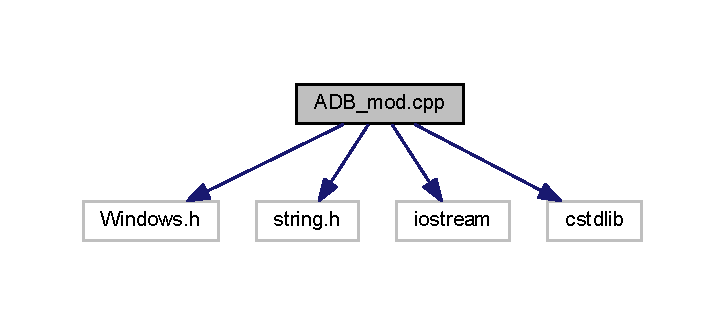
\includegraphics[width=348pt]{_a_d_b__mod_8cpp__incl}
\end{center}
\end{figure}
\subsection*{Функции}
\begin{DoxyCompactItemize}
\item 
void \hyperlink{_a_d_b__mod_8cpp_a5d0a3a01ef690bcd93495becd3273063}{adb} (L\+P\+S\+TR cmd\+Args)
\item 
void \hyperlink{_a_d_b__mod_8cpp_a3b7f80fa75c7705429c3d7402fec0eb0}{fastboot} (L\+P\+S\+TR cmd\+Args)
\end{DoxyCompactItemize}


\subsection{Подробное описание}
Модуль работы с adb. 

\begin{DoxyAuthor}{Автор}
Darlakon 
\end{DoxyAuthor}


\subsection{Функции}
\mbox{\Hypertarget{_a_d_b__mod_8cpp_a5d0a3a01ef690bcd93495becd3273063}\label{_a_d_b__mod_8cpp_a5d0a3a01ef690bcd93495becd3273063}} 
\index{A\+D\+B\+\_\+mod.\+cpp@{A\+D\+B\+\_\+mod.\+cpp}!adb@{adb}}
\index{adb@{adb}!A\+D\+B\+\_\+mod.\+cpp@{A\+D\+B\+\_\+mod.\+cpp}}
\subsubsection{\texorpdfstring{adb()}{adb()}}
{\footnotesize\ttfamily void adb (\begin{DoxyParamCaption}\item[{L\+P\+S\+TR}]{cmd\+Args }\end{DoxyParamCaption})}

Вызов adb-\/интерфейса. 
\begin{DoxyParams}[1]{Аргументы}
\mbox{\tt in}  & {\em cmd\+Args} & -\/ команда для adb вида \char`\"{}adb X\char`\"{}. \\
\hline
\end{DoxyParams}


См. определение в файле A\+D\+B\+\_\+mod.\+cpp строка 16

\mbox{\Hypertarget{_a_d_b__mod_8cpp_a3b7f80fa75c7705429c3d7402fec0eb0}\label{_a_d_b__mod_8cpp_a3b7f80fa75c7705429c3d7402fec0eb0}} 
\index{A\+D\+B\+\_\+mod.\+cpp@{A\+D\+B\+\_\+mod.\+cpp}!fastboot@{fastboot}}
\index{fastboot@{fastboot}!A\+D\+B\+\_\+mod.\+cpp@{A\+D\+B\+\_\+mod.\+cpp}}
\subsubsection{\texorpdfstring{fastboot()}{fastboot()}}
{\footnotesize\ttfamily void fastboot (\begin{DoxyParamCaption}\item[{L\+P\+S\+TR}]{cmd\+Args }\end{DoxyParamCaption})}

Вызов fastboot-\/интерфейса. 
\begin{DoxyParams}[1]{Аргументы}
\mbox{\tt in}  & {\em cmd\+Args} & -\/ команда для fastboot вида \char`\"{}fastboot X\char`\"{}. \\
\hline
\end{DoxyParams}


См. определение в файле A\+D\+B\+\_\+mod.\+cpp строка 40


\hypertarget{_a_d_b__mod_8h}{}\section{Файл A\+D\+B\+\_\+mod.\+h}
\label{_a_d_b__mod_8h}\index{A\+D\+B\+\_\+mod.\+h@{A\+D\+B\+\_\+mod.\+h}}


Заголовочный файл с подключением модуля работы с adb.  


{\ttfamily \#include $<$Windows.\+h$>$}\newline
Граф включаемых заголовочных файлов для A\+D\+B\+\_\+mod.\+h\+:
\nopagebreak
\begin{figure}[H]
\begin{center}
\leavevmode
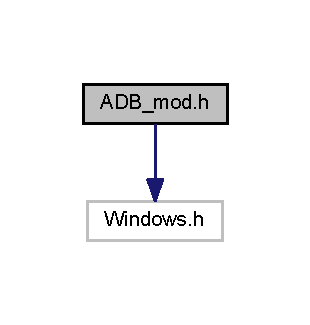
\includegraphics[width=149pt]{_a_d_b__mod_8h__incl}
\end{center}
\end{figure}
Граф файлов, в которые включается этот файл\+:
\nopagebreak
\begin{figure}[H]
\begin{center}
\leavevmode
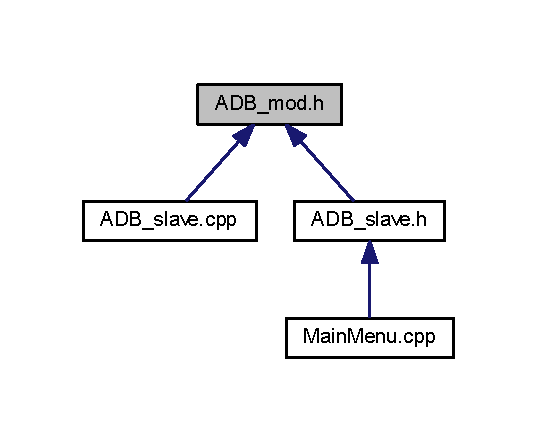
\includegraphics[width=258pt]{_a_d_b__mod_8h__dep__incl}
\end{center}
\end{figure}
\subsection*{Функции}
\begin{DoxyCompactItemize}
\item 
int \hyperlink{_a_d_b__mod_8h_a19cfc330dc0bc3b0d13655568b86ef45}{adb} (L\+P\+S\+TR cmd\+Args)
\item 
int \hyperlink{_a_d_b__mod_8h_a0cc4e45f70c18d1e0a8d552fa8c821b6}{fastboot} (L\+P\+S\+TR cmd\+Args)
\end{DoxyCompactItemize}


\subsection{Подробное описание}
Заголовочный файл с подключением модуля работы с adb. 

\begin{DoxyAuthor}{Автор}
Darlakon 
\end{DoxyAuthor}


\subsection{Функции}
\mbox{\Hypertarget{_a_d_b__mod_8h_a19cfc330dc0bc3b0d13655568b86ef45}\label{_a_d_b__mod_8h_a19cfc330dc0bc3b0d13655568b86ef45}} 
\index{A\+D\+B\+\_\+mod.\+h@{A\+D\+B\+\_\+mod.\+h}!adb@{adb}}
\index{adb@{adb}!A\+D\+B\+\_\+mod.\+h@{A\+D\+B\+\_\+mod.\+h}}
\subsubsection{\texorpdfstring{adb()}{adb()}}
{\footnotesize\ttfamily int adb (\begin{DoxyParamCaption}\item[{L\+P\+S\+TR}]{cmd\+Args }\end{DoxyParamCaption})}

Вызов adb-\/интерфейса. L\+P\+S\+TR cmd\+Args -\/ команда для adb вида \char`\"{}adb X\char`\"{}. 

См. определение в файле A\+D\+B\+\_\+mod.\+cpp строка 11

\mbox{\Hypertarget{_a_d_b__mod_8h_a0cc4e45f70c18d1e0a8d552fa8c821b6}\label{_a_d_b__mod_8h_a0cc4e45f70c18d1e0a8d552fa8c821b6}} 
\index{A\+D\+B\+\_\+mod.\+h@{A\+D\+B\+\_\+mod.\+h}!fastboot@{fastboot}}
\index{fastboot@{fastboot}!A\+D\+B\+\_\+mod.\+h@{A\+D\+B\+\_\+mod.\+h}}
\subsubsection{\texorpdfstring{fastboot()}{fastboot()}}
{\footnotesize\ttfamily int fastboot (\begin{DoxyParamCaption}\item[{L\+P\+S\+TR}]{cmd\+Args }\end{DoxyParamCaption})}

Вызов fastboot-\/интерфейса. L\+P\+S\+TR cmd\+Args -\/ команда для fastboot вида \char`\"{}fastboot X\char`\"{}. 

См. определение в файле A\+D\+B\+\_\+mod.\+cpp строка 36


\hypertarget{_a_d_b__slave_8cpp}{}\section{Файл A\+D\+B\+\_\+slave.\+cpp}
\label{_a_d_b__slave_8cpp}\index{A\+D\+B\+\_\+slave.\+cpp@{A\+D\+B\+\_\+slave.\+cpp}}
{\ttfamily \#include \char`\"{}A\+D\+B\+\_\+mod.\+h\char`\"{}}\newline
Граф включаемых заголовочных файлов для A\+D\+B\+\_\+slave.\+cpp\+:
\nopagebreak
\begin{figure}[H]
\begin{center}
\leavevmode
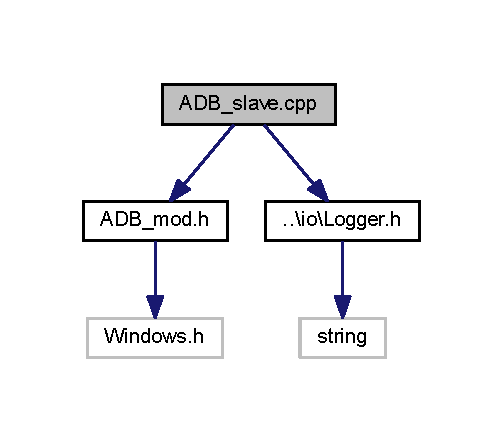
\includegraphics[width=163pt]{_a_d_b__slave_8cpp__incl}
\end{center}
\end{figure}
\subsection*{Функции}
\begin{DoxyCompactItemize}
\item 
void \hyperlink{_a_d_b__slave_8cpp_ad1f1e991625b5f039ea46c20d003ed0f}{adb\+\_\+state} ()
\item 
void \hyperlink{_a_d_b__slave_8cpp_a6b830192de1fd9a84e95434750984282}{adb\+\_\+flash} ()
\item 
void \hyperlink{_a_d_b__slave_8cpp_abe46e301720694fb6fcec4868d54f516}{adb\+\_\+root} ()
\end{DoxyCompactItemize}


\subsection{Функции}
\mbox{\Hypertarget{_a_d_b__slave_8cpp_a6b830192de1fd9a84e95434750984282}\label{_a_d_b__slave_8cpp_a6b830192de1fd9a84e95434750984282}} 
\index{A\+D\+B\+\_\+slave.\+cpp@{A\+D\+B\+\_\+slave.\+cpp}!adb\+\_\+flash@{adb\+\_\+flash}}
\index{adb\+\_\+flash@{adb\+\_\+flash}!A\+D\+B\+\_\+slave.\+cpp@{A\+D\+B\+\_\+slave.\+cpp}}
\subsubsection{\texorpdfstring{adb\+\_\+flash()}{adb\_flash()}}
{\footnotesize\ttfamily void adb\+\_\+flash (\begin{DoxyParamCaption}{ }\end{DoxyParamCaption})}

Вызов модуля установки кастомной рекавери. Требуется экстремальный пересмотр, ничего не работает. 

См. определение в файле A\+D\+B\+\_\+slave.\+cpp строка 15

\mbox{\Hypertarget{_a_d_b__slave_8cpp_abe46e301720694fb6fcec4868d54f516}\label{_a_d_b__slave_8cpp_abe46e301720694fb6fcec4868d54f516}} 
\index{A\+D\+B\+\_\+slave.\+cpp@{A\+D\+B\+\_\+slave.\+cpp}!adb\+\_\+root@{adb\+\_\+root}}
\index{adb\+\_\+root@{adb\+\_\+root}!A\+D\+B\+\_\+slave.\+cpp@{A\+D\+B\+\_\+slave.\+cpp}}
\subsubsection{\texorpdfstring{adb\+\_\+root()}{adb\_root()}}
{\footnotesize\ttfamily void adb\+\_\+root (\begin{DoxyParamCaption}{ }\end{DoxyParamCaption})}

Вызов модуля получения root-\/прав. Требуется тестирование на работоспособность. 

См. определение в файле A\+D\+B\+\_\+slave.\+cpp строка 30

\mbox{\Hypertarget{_a_d_b__slave_8cpp_ad1f1e991625b5f039ea46c20d003ed0f}\label{_a_d_b__slave_8cpp_ad1f1e991625b5f039ea46c20d003ed0f}} 
\index{A\+D\+B\+\_\+slave.\+cpp@{A\+D\+B\+\_\+slave.\+cpp}!adb\+\_\+state@{adb\+\_\+state}}
\index{adb\+\_\+state@{adb\+\_\+state}!A\+D\+B\+\_\+slave.\+cpp@{A\+D\+B\+\_\+slave.\+cpp}}
\subsubsection{\texorpdfstring{adb\+\_\+state()}{adb\_state()}}
{\footnotesize\ttfamily void adb\+\_\+state (\begin{DoxyParamCaption}{ }\end{DoxyParamCaption})}

Вызов модуля проверки состояния устройства. 

См. определение в файле A\+D\+B\+\_\+slave.\+cpp строка 6


\hypertarget{_a_d_b__slave_8h}{}\section{Файл A\+D\+B\+\_\+slave.\+h}
\label{_a_d_b__slave_8h}\index{A\+D\+B\+\_\+slave.\+h@{A\+D\+B\+\_\+slave.\+h}}


Заголовочный файл с подключением модуля работы с adb.  


{\ttfamily \#include \char`\"{}..\textbackslash{}core\textbackslash{}\+A\+D\+B\+\_\+mod.\+h\char`\"{}}\newline
Граф включаемых заголовочных файлов для A\+D\+B\+\_\+slave.\+h\+:
\nopagebreak
\begin{figure}[H]
\begin{center}
\leavevmode
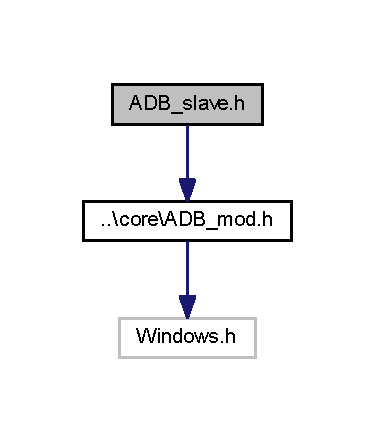
\includegraphics[width=180pt]{_a_d_b__slave_8h__incl}
\end{center}
\end{figure}
Граф файлов, в которые включается этот файл\+:
\nopagebreak
\begin{figure}[H]
\begin{center}
\leavevmode
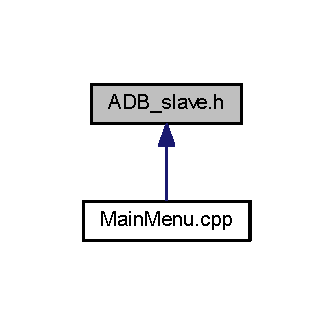
\includegraphics[width=160pt]{_a_d_b__slave_8h__dep__incl}
\end{center}
\end{figure}
\subsection*{Функции}
\begin{DoxyCompactItemize}
\item 
void \hyperlink{_a_d_b__slave_8h_ad1f1e991625b5f039ea46c20d003ed0f}{adb\+\_\+state} ()
\item 
void \hyperlink{_a_d_b__slave_8h_a6b830192de1fd9a84e95434750984282}{adb\+\_\+flash} ()
\item 
void \hyperlink{_a_d_b__slave_8h_abe46e301720694fb6fcec4868d54f516}{adb\+\_\+root} ()
\end{DoxyCompactItemize}


\subsection{Подробное описание}
Заголовочный файл с подключением модуля работы с adb. 

\begin{DoxyAuthor}{Автор}
Darlakon 
\end{DoxyAuthor}


\subsection{Функции}
\mbox{\Hypertarget{_a_d_b__slave_8h_a6b830192de1fd9a84e95434750984282}\label{_a_d_b__slave_8h_a6b830192de1fd9a84e95434750984282}} 
\index{A\+D\+B\+\_\+slave.\+h@{A\+D\+B\+\_\+slave.\+h}!adb\+\_\+flash@{adb\+\_\+flash}}
\index{adb\+\_\+flash@{adb\+\_\+flash}!A\+D\+B\+\_\+slave.\+h@{A\+D\+B\+\_\+slave.\+h}}
\subsubsection{\texorpdfstring{adb\+\_\+flash()}{adb\_flash()}}
{\footnotesize\ttfamily void adb\+\_\+flash (\begin{DoxyParamCaption}{ }\end{DoxyParamCaption})}

Вызов модуля установки кастомной рекавери.

Вызов модуля установки кастомной рекавери. Требуется экстремальный пересмотр, ничего не работает. 

См. определение в файле A\+D\+B\+\_\+slave.\+cpp строка 15

\mbox{\Hypertarget{_a_d_b__slave_8h_abe46e301720694fb6fcec4868d54f516}\label{_a_d_b__slave_8h_abe46e301720694fb6fcec4868d54f516}} 
\index{A\+D\+B\+\_\+slave.\+h@{A\+D\+B\+\_\+slave.\+h}!adb\+\_\+root@{adb\+\_\+root}}
\index{adb\+\_\+root@{adb\+\_\+root}!A\+D\+B\+\_\+slave.\+h@{A\+D\+B\+\_\+slave.\+h}}
\subsubsection{\texorpdfstring{adb\+\_\+root()}{adb\_root()}}
{\footnotesize\ttfamily void adb\+\_\+root (\begin{DoxyParamCaption}{ }\end{DoxyParamCaption})}

Вызов модуля получения root-\/прав.

Вызов модуля получения root-\/прав. Требуется тестирование на работоспособность. 

См. определение в файле A\+D\+B\+\_\+slave.\+cpp строка 30

\mbox{\Hypertarget{_a_d_b__slave_8h_ad1f1e991625b5f039ea46c20d003ed0f}\label{_a_d_b__slave_8h_ad1f1e991625b5f039ea46c20d003ed0f}} 
\index{A\+D\+B\+\_\+slave.\+h@{A\+D\+B\+\_\+slave.\+h}!adb\+\_\+state@{adb\+\_\+state}}
\index{adb\+\_\+state@{adb\+\_\+state}!A\+D\+B\+\_\+slave.\+h@{A\+D\+B\+\_\+slave.\+h}}
\subsubsection{\texorpdfstring{adb\+\_\+state()}{adb\_state()}}
{\footnotesize\ttfamily void adb\+\_\+state (\begin{DoxyParamCaption}{ }\end{DoxyParamCaption})}

Вызов модуля проверки состояния устройства. 

См. определение в файле A\+D\+B\+\_\+slave.\+cpp строка 6


\hypertarget{_check_agreement_8cpp}{}\section{Файл Check\+Agreement.\+cpp}
\label{_check_agreement_8cpp}\index{Check\+Agreement.\+cpp@{Check\+Agreement.\+cpp}}


Модуль проверки согласия пользователя с правилами.  


{\ttfamily \#include $<$iostream$>$}\newline
{\ttfamily \#include $<$conio.\+h$>$}\newline
{\ttfamily \#include $<$string$>$}\newline
{\ttfamily \#include \char`\"{}..\textbackslash{}core\textbackslash{}\+Color.\+h\char`\"{}}\newline
{\ttfamily \#include \char`\"{}..\textbackslash{}core\textbackslash{}\+Logo.\+h\char`\"{}}\newline
{\ttfamily \#include \char`\"{}..\textbackslash{}core\textbackslash{}\+Constants\+Menu.\+h\char`\"{}}\newline
{\ttfamily \#include \char`\"{}..\textbackslash{}io\textbackslash{}\+Rules\+List.\+h\char`\"{}}\newline
Граф включаемых заголовочных файлов для Check\+Agreement.\+cpp\+:
\nopagebreak
\begin{figure}[H]
\begin{center}
\leavevmode
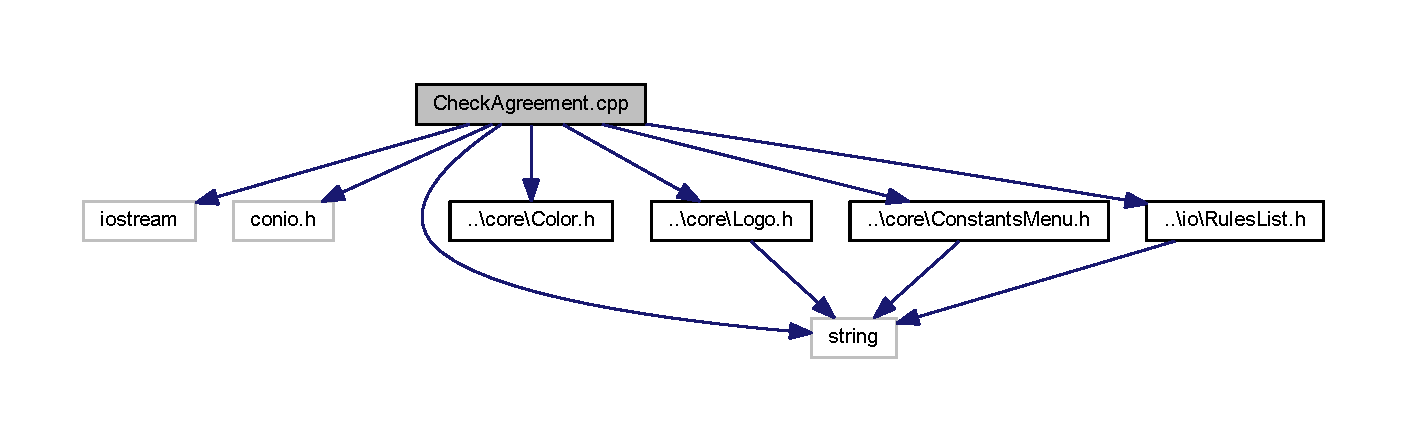
\includegraphics[width=350pt]{_check_agreement_8cpp__incl}
\end{center}
\end{figure}
\subsection*{Функции}
\begin{DoxyCompactItemize}
\item 
void \hyperlink{_check_agreement_8cpp_acf2bff465d8177c63f6904d73e1cafdf}{v\+\_\+checkagreement\+\_\+choice} (size\+\_\+t choice)
\item 
int \hyperlink{_check_agreement_8cpp_a3d3fea8d8c6da49b2f73fc0b2c2e7574}{i\+\_\+checkagreement} ()
\end{DoxyCompactItemize}


\subsection{Подробное описание}
Модуль проверки согласия пользователя с правилами. 

\begin{DoxyAuthor}{Автор}
Sava\+Lione 
\end{DoxyAuthor}


\subsection{Функции}
\mbox{\Hypertarget{_check_agreement_8cpp_a3d3fea8d8c6da49b2f73fc0b2c2e7574}\label{_check_agreement_8cpp_a3d3fea8d8c6da49b2f73fc0b2c2e7574}} 
\index{Check\+Agreement.\+cpp@{Check\+Agreement.\+cpp}!i\+\_\+checkagreement@{i\+\_\+checkagreement}}
\index{i\+\_\+checkagreement@{i\+\_\+checkagreement}!Check\+Agreement.\+cpp@{Check\+Agreement.\+cpp}}
\subsubsection{\texorpdfstring{i\+\_\+checkagreement()}{i\_checkagreement()}}
{\footnotesize\ttfamily int i\+\_\+checkagreement (\begin{DoxyParamCaption}{ }\end{DoxyParamCaption})}

Вызов модуля проверки согласия пользователя с правилами. \begin{DoxyReturn}{Возвращает}
0 -\/ пользователь не согласен с условиями программы, выход из программы. 1 -\/ пользователь согласен с условиями программы, запуск программы. 
\end{DoxyReturn}


См. определение в файле Check\+Agreement.\+cpp строка 47

\mbox{\Hypertarget{_check_agreement_8cpp_acf2bff465d8177c63f6904d73e1cafdf}\label{_check_agreement_8cpp_acf2bff465d8177c63f6904d73e1cafdf}} 
\index{Check\+Agreement.\+cpp@{Check\+Agreement.\+cpp}!v\+\_\+checkagreement\+\_\+choice@{v\+\_\+checkagreement\+\_\+choice}}
\index{v\+\_\+checkagreement\+\_\+choice@{v\+\_\+checkagreement\+\_\+choice}!Check\+Agreement.\+cpp@{Check\+Agreement.\+cpp}}
\subsubsection{\texorpdfstring{v\+\_\+checkagreement\+\_\+choice()}{v\_checkagreement\_choice()}}
{\footnotesize\ttfamily void v\+\_\+checkagreement\+\_\+choice (\begin{DoxyParamCaption}\item[{size\+\_\+t}]{choice }\end{DoxyParamCaption})}

Переключение пунктов меню 
\begin{DoxyParams}[1]{Аргументы}
\mbox{\tt in}  & {\em choice} & выбор \\
\hline
\end{DoxyParams}


См. определение в файле Check\+Agreement.\+cpp строка 22


\hypertarget{_check_agreement_8h}{}\section{Файл Check\+Agreement.\+h}
\label{_check_agreement_8h}\index{Check\+Agreement.\+h@{Check\+Agreement.\+h}}


Заголовочный файл с подключением модуля проверки согласия с лицензией.  


Граф файлов, в которые включается этот файл\+:
\nopagebreak
\begin{figure}[H]
\begin{center}
\leavevmode
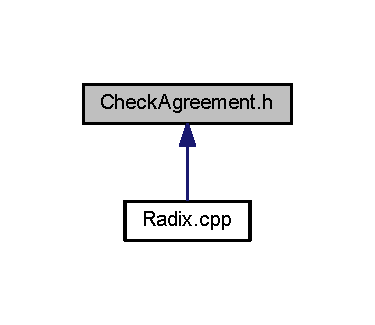
\includegraphics[width=180pt]{_check_agreement_8h__dep__incl}
\end{center}
\end{figure}
\subsection*{Функции}
\begin{DoxyCompactItemize}
\item 
int \hyperlink{_check_agreement_8h_a3d3fea8d8c6da49b2f73fc0b2c2e7574}{i\+\_\+checkagreement} ()
\end{DoxyCompactItemize}


\subsection{Подробное описание}
Заголовочный файл с подключением модуля проверки согласия с лицензией. 

\begin{DoxyAuthor}{Автор}
Sava\+Lione 
\end{DoxyAuthor}


\subsection{Функции}
\mbox{\Hypertarget{_check_agreement_8h_a3d3fea8d8c6da49b2f73fc0b2c2e7574}\label{_check_agreement_8h_a3d3fea8d8c6da49b2f73fc0b2c2e7574}} 
\index{Check\+Agreement.\+h@{Check\+Agreement.\+h}!i\+\_\+checkagreement@{i\+\_\+checkagreement}}
\index{i\+\_\+checkagreement@{i\+\_\+checkagreement}!Check\+Agreement.\+h@{Check\+Agreement.\+h}}
\subsubsection{\texorpdfstring{i\+\_\+checkagreement()}{i\_checkagreement()}}
{\footnotesize\ttfamily int i\+\_\+checkagreement (\begin{DoxyParamCaption}{ }\end{DoxyParamCaption})}

Вызов модуля проверки согласия пользователя с правилами. \begin{DoxyReturn}{Возвращает}
0 -\/ пользователь не согласен с условиями программы, выход из программы. 1 -\/ пользователь согласен с условиями программы, запуск программы. 
\end{DoxyReturn}


См. определение в файле Check\+Agreement.\+cpp строка 66


\hypertarget{_color_8cpp}{}\section{Файл Color.\+cpp}
\label{_color_8cpp}\index{Color.\+cpp@{Color.\+cpp}}


Модуль работы с цветом в консоли.  


{\ttfamily \#include $<$windows.\+h$>$}\newline
{\ttfamily \#include $<$iostream$>$}\newline
{\ttfamily \#include \char`\"{}Color.\+h\char`\"{}}\newline
Граф включаемых заголовочных файлов для Color.\+cpp\+:
\nopagebreak
\begin{figure}[H]
\begin{center}
\leavevmode
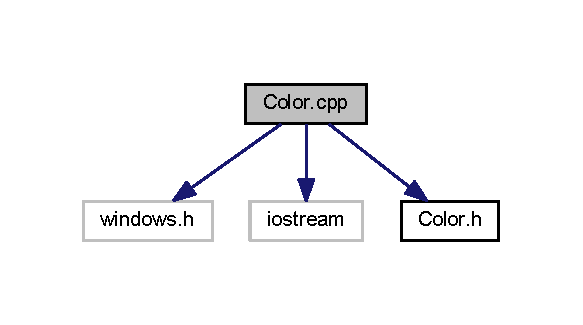
\includegraphics[width=280pt]{_color_8cpp__incl}
\end{center}
\end{figure}
\subsection*{Функции}
\begin{DoxyCompactItemize}
\item 
void \hyperlink{_color_8cpp_a8bfe4542d1f10bae3f4ff0ec688aa67f}{v\+\_\+set\+\_\+color} (\hyperlink{_color_8h_a37dbdc30935031c05304482e1be89d8f}{color} Console\+Text, \hyperlink{_color_8h_a37dbdc30935031c05304482e1be89d8f}{color} Console\+Background)
\item 
void \hyperlink{_color_8cpp_ac4b485399ce8f366e640bbfe8ea40f7b}{v\+\_\+set\+\_\+color} (\hyperlink{_color_8h_a37dbdc30935031c05304482e1be89d8f}{color} Console\+Text)
\item 
void \hyperlink{_color_8cpp_a6ef2ca7a5d188bef59eb0af85f5509ec}{v\+\_\+set\+\_\+color} ()
\end{DoxyCompactItemize}


\subsection{Подробное описание}
Модуль работы с цветом в консоли. 

Модуль позволяет менять цвет текста и цвет фона в консоли.

\begin{DoxyAuthor}{Автор}
Sava\+Lione 
\end{DoxyAuthor}


\subsection{Функции}
\mbox{\Hypertarget{_color_8cpp_a8bfe4542d1f10bae3f4ff0ec688aa67f}\label{_color_8cpp_a8bfe4542d1f10bae3f4ff0ec688aa67f}} 
\index{Color.\+cpp@{Color.\+cpp}!v\+\_\+set\+\_\+color@{v\+\_\+set\+\_\+color}}
\index{v\+\_\+set\+\_\+color@{v\+\_\+set\+\_\+color}!Color.\+cpp@{Color.\+cpp}}
\subsubsection{\texorpdfstring{v\+\_\+set\+\_\+color()}{v\_set\_color()}\hspace{0.1cm}{\footnotesize\ttfamily [1/3]}}
{\footnotesize\ttfamily void v\+\_\+set\+\_\+color (\begin{DoxyParamCaption}\item[{\hyperlink{_color_8h_a37dbdc30935031c05304482e1be89d8f}{color}}]{Console\+Text,  }\item[{\hyperlink{_color_8h_a37dbdc30935031c05304482e1be89d8f}{color}}]{Console\+Background }\end{DoxyParamCaption})}

Изменение цвета текста и цвета заднего фона в консоли 
\begin{DoxyParams}[1]{Аргументы}
\mbox{\tt in}  & {\em Console\+Text} & цвет текста \\
\hline
\mbox{\tt in}  & {\em Console\+Background} & цвет заднего фона \\
\hline
\end{DoxyParams}


См. определение в файле Color.\+cpp строка 20

\mbox{\Hypertarget{_color_8cpp_ac4b485399ce8f366e640bbfe8ea40f7b}\label{_color_8cpp_ac4b485399ce8f366e640bbfe8ea40f7b}} 
\index{Color.\+cpp@{Color.\+cpp}!v\+\_\+set\+\_\+color@{v\+\_\+set\+\_\+color}}
\index{v\+\_\+set\+\_\+color@{v\+\_\+set\+\_\+color}!Color.\+cpp@{Color.\+cpp}}
\subsubsection{\texorpdfstring{v\+\_\+set\+\_\+color()}{v\_set\_color()}\hspace{0.1cm}{\footnotesize\ttfamily [2/3]}}
{\footnotesize\ttfamily void v\+\_\+set\+\_\+color (\begin{DoxyParamCaption}\item[{\hyperlink{_color_8h_a37dbdc30935031c05304482e1be89d8f}{color}}]{Console\+Text }\end{DoxyParamCaption})}

Изменение цвета текста в консоли. Задний фон по умолчанию чёрный. 
\begin{DoxyParams}[1]{Аргументы}
\mbox{\tt in}  & {\em Console\+Text} & цвет текста \\
\hline
\end{DoxyParams}


См. определение в файле Color.\+cpp строка 28

\mbox{\Hypertarget{_color_8cpp_a6ef2ca7a5d188bef59eb0af85f5509ec}\label{_color_8cpp_a6ef2ca7a5d188bef59eb0af85f5509ec}} 
\index{Color.\+cpp@{Color.\+cpp}!v\+\_\+set\+\_\+color@{v\+\_\+set\+\_\+color}}
\index{v\+\_\+set\+\_\+color@{v\+\_\+set\+\_\+color}!Color.\+cpp@{Color.\+cpp}}
\subsubsection{\texorpdfstring{v\+\_\+set\+\_\+color()}{v\_set\_color()}\hspace{0.1cm}{\footnotesize\ttfamily [3/3]}}
{\footnotesize\ttfamily void v\+\_\+set\+\_\+color (\begin{DoxyParamCaption}{ }\end{DoxyParamCaption})}

Вернуть цвет текста и цвет заднего фона в консоли к стандартным значениям. 

См. определение в файле Color.\+cpp строка 34


\hypertarget{_color_8h}{}\section{Файл Color.\+h}
\label{_color_8h}\index{Color.\+h@{Color.\+h}}


Заголовочный файл с цветами и модулем смены цвета в консоли.  


Граф файлов, в которые включается этот файл\+:\nopagebreak
\begin{figure}[H]
\begin{center}
\leavevmode
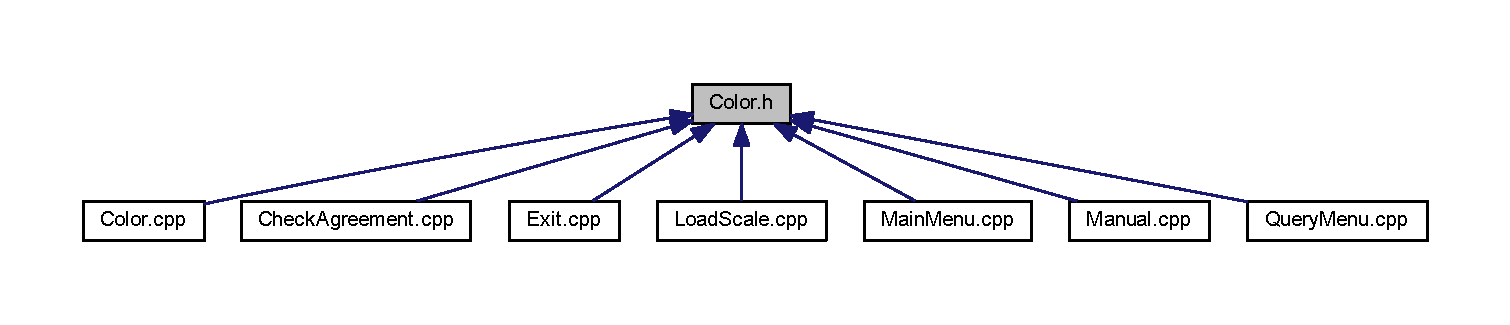
\includegraphics[width=350pt]{_color_8h__dep__incl}
\end{center}
\end{figure}
\subsection*{Перечисления}
\begin{DoxyCompactItemize}
\item 
enum \hyperlink{_color_8h_a37dbdc30935031c05304482e1be89d8f}{color} \{ \newline
{\bfseries B\+L\+A\+CK} = 0, 
{\bfseries B\+L\+UE} = 1, 
{\bfseries G\+R\+E\+EN} = 2, 
{\bfseries C\+Y\+AN} = 3, 
\newline
{\bfseries R\+ED} = 4, 
{\bfseries M\+A\+G\+E\+N\+TA} = 5, 
{\bfseries B\+R\+O\+WN} = 6, 
{\bfseries L\+I\+G\+H\+T\+G\+R\+AY} = 7, 
\newline
{\bfseries D\+A\+R\+K\+G\+R\+AY} = 8, 
{\bfseries L\+I\+G\+H\+T\+B\+L\+UE} = 9, 
{\bfseries L\+I\+G\+H\+T\+G\+R\+E\+EN} = 10, 
{\bfseries L\+I\+G\+H\+T\+C\+Y\+AN} = 11, 
\newline
{\bfseries L\+I\+G\+H\+T\+R\+ED} = 12, 
{\bfseries L\+I\+G\+H\+T\+M\+A\+G\+E\+N\+TA} = 13, 
{\bfseries L\+I\+G\+H\+T\+Y\+E\+L\+L\+OW} = 14, 
{\bfseries W\+H\+I\+TE} = 15
 \}
\end{DoxyCompactItemize}
\subsection*{Функции}
\begin{DoxyCompactItemize}
\item 
void \hyperlink{_color_8h_a8bfe4542d1f10bae3f4ff0ec688aa67f}{v\+\_\+set\+\_\+color} (\hyperlink{_color_8h_a37dbdc30935031c05304482e1be89d8f}{color} Console\+Text, \hyperlink{_color_8h_a37dbdc30935031c05304482e1be89d8f}{color} Console\+Background)
\item 
void \hyperlink{_color_8h_ac4b485399ce8f366e640bbfe8ea40f7b}{v\+\_\+set\+\_\+color} (\hyperlink{_color_8h_a37dbdc30935031c05304482e1be89d8f}{color} Console\+Text)
\item 
void \hyperlink{_color_8h_a6ef2ca7a5d188bef59eb0af85f5509ec}{v\+\_\+set\+\_\+color} ()
\end{DoxyCompactItemize}


\subsection{Подробное описание}
Заголовочный файл с цветами и модулем смены цвета в консоли. 

\begin{DoxyAuthor}{Автор}
Sava\+Lione 
\end{DoxyAuthor}


\subsection{Перечисления}
\mbox{\Hypertarget{_color_8h_a37dbdc30935031c05304482e1be89d8f}\label{_color_8h_a37dbdc30935031c05304482e1be89d8f}} 
\index{Color.\+h@{Color.\+h}!color@{color}}
\index{color@{color}!Color.\+h@{Color.\+h}}
\subsubsection{\texorpdfstring{color}{color}}
{\footnotesize\ttfamily enum \hyperlink{_color_8h_a37dbdc30935031c05304482e1be89d8f}{color}}

Цвета 

\subsection{Функции}
\mbox{\Hypertarget{_color_8h_a8bfe4542d1f10bae3f4ff0ec688aa67f}\label{_color_8h_a8bfe4542d1f10bae3f4ff0ec688aa67f}} 
\index{Color.\+h@{Color.\+h}!v\+\_\+set\+\_\+color@{v\+\_\+set\+\_\+color}}
\index{v\+\_\+set\+\_\+color@{v\+\_\+set\+\_\+color}!Color.\+h@{Color.\+h}}
\subsubsection{\texorpdfstring{v\+\_\+set\+\_\+color()}{v\_set\_color()}\hspace{0.1cm}{\footnotesize\ttfamily [1/3]}}
{\footnotesize\ttfamily void v\+\_\+set\+\_\+color (\begin{DoxyParamCaption}\item[{\hyperlink{_color_8h_a37dbdc30935031c05304482e1be89d8f}{color}}]{Console\+Text,  }\item[{\hyperlink{_color_8h_a37dbdc30935031c05304482e1be89d8f}{color}}]{Console\+Background }\end{DoxyParamCaption})}

Изменение цвета текста и цвета заднего фона в консоли 
\begin{DoxyParams}[1]{Аргументы}
\mbox{\tt in}  & {\em Console\+Text} & цвет текста \\
\hline
\mbox{\tt in}  & {\em Console\+Background} & цвет заднего фона \\
\hline
\end{DoxyParams}
\mbox{\Hypertarget{_color_8h_ac4b485399ce8f366e640bbfe8ea40f7b}\label{_color_8h_ac4b485399ce8f366e640bbfe8ea40f7b}} 
\index{Color.\+h@{Color.\+h}!v\+\_\+set\+\_\+color@{v\+\_\+set\+\_\+color}}
\index{v\+\_\+set\+\_\+color@{v\+\_\+set\+\_\+color}!Color.\+h@{Color.\+h}}
\subsubsection{\texorpdfstring{v\+\_\+set\+\_\+color()}{v\_set\_color()}\hspace{0.1cm}{\footnotesize\ttfamily [2/3]}}
{\footnotesize\ttfamily void v\+\_\+set\+\_\+color (\begin{DoxyParamCaption}\item[{\hyperlink{_color_8h_a37dbdc30935031c05304482e1be89d8f}{color}}]{Console\+Text }\end{DoxyParamCaption})}

Изменение цвета текста в консоли. Задний фон по умолчанию чёрный. 
\begin{DoxyParams}[1]{Аргументы}
\mbox{\tt in}  & {\em Console\+Text} & цвет текста \\
\hline
\end{DoxyParams}
\mbox{\Hypertarget{_color_8h_a6ef2ca7a5d188bef59eb0af85f5509ec}\label{_color_8h_a6ef2ca7a5d188bef59eb0af85f5509ec}} 
\index{Color.\+h@{Color.\+h}!v\+\_\+set\+\_\+color@{v\+\_\+set\+\_\+color}}
\index{v\+\_\+set\+\_\+color@{v\+\_\+set\+\_\+color}!Color.\+h@{Color.\+h}}
\subsubsection{\texorpdfstring{v\+\_\+set\+\_\+color()}{v\_set\_color()}\hspace{0.1cm}{\footnotesize\ttfamily [3/3]}}
{\footnotesize\ttfamily void v\+\_\+set\+\_\+color (\begin{DoxyParamCaption}{ }\end{DoxyParamCaption})}

Вернуть цвет текста и цвет заднего фона в консоли к стандартным значениям. 
\hypertarget{_constants_8h}{}\section{Файл Constants.\+h}
\label{_constants_8h}\index{Constants.\+h@{Constants.\+h}}


Заголовочный файл с константами.  


Граф файлов, в которые включается этот файл\+:
\nopagebreak
\begin{figure}[H]
\begin{center}
\leavevmode
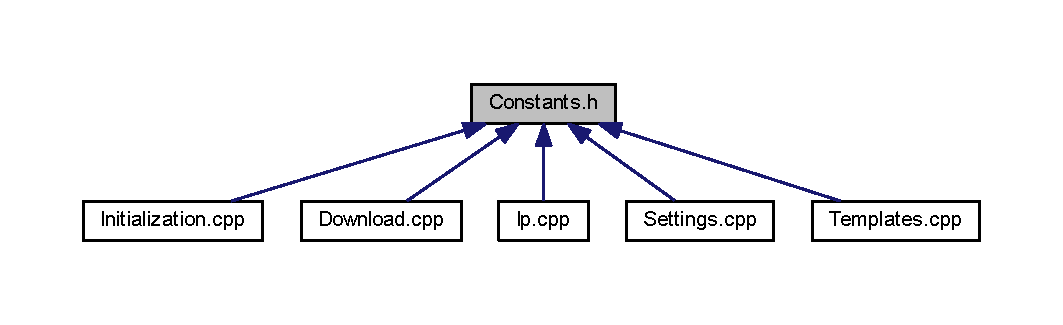
\includegraphics[width=350pt]{_constants_8h__dep__incl}
\end{center}
\end{figure}
\subsection*{Пространства имен}
\begin{DoxyCompactItemize}
\item 
 \hyperlink{namespaceradix}{radix}
\end{DoxyCompactItemize}
\subsection*{Переменные}
\begin{DoxyCompactItemize}
\item 
const size\+\_\+t \hyperlink{namespaceradix_a82e81e89088b6430b7ec11a8a0329e9c}{radix\+::buff\+\_\+size} = 32
\item 
const size\+\_\+t \hyperlink{namespaceradix_a8f000aabf647d34fd877c33958bad711}{radix\+::buff\+\_\+ruleslist} = 256
\item 
const char \hyperlink{namespaceradix_a11c5bfe5c65a0f88a2a950111c6ffc09}{radix\+::logger\+\_\+list} \mbox{[}$\,$\mbox{]} = \char`\"{}logger.\+log\char`\"{}
\item 
const char \hyperlink{namespaceradix_a43bff57dbd1b7dcebee0228ccbab7f17}{radix\+::settings\+\_\+list} \mbox{[}$\,$\mbox{]} = \char`\"{}settings.\+ini\char`\"{}
\item 
const char \hyperlink{namespaceradix_a73b088a3e903cc2845c2299b9ab8ccaf}{radix\+::rules\+\_\+list} \mbox{[}$\,$\mbox{]} = \char`\"{}rules.\+txt\char`\"{}
\item 
const char \hyperlink{namespaceradix_a123392a7ece6e11efaf3ad3df291ff3d}{radix\+::firmware\+\_\+way} \mbox{[}$\,$\mbox{]} = \char`\"{}\textbackslash{}\textbackslash{}assets\textbackslash{}\textbackslash{}firmware\textbackslash{}\textbackslash{}\char`\"{}
\item 
const char \hyperlink{namespaceradix_aa90f63f1d0143b58469670ccbb86cfc4}{radix\+::patch} \mbox{[}$\,$\mbox{]} = \char`\"{}\textbackslash{}\textbackslash{}assets\textbackslash{}\textbackslash{}\char`\"{}
\item 
const char \hyperlink{namespaceradix_a01a09f0b88f6fd375ea20667bd318035}{radix\+::expansion\+\_\+file} \mbox{[}$\,$\mbox{]} = \char`\"{}.zip\char`\"{}
\item 
const char \hyperlink{namespaceradix_a91c21d6be385236a564ef5bf1f3f3602}{radix\+::recovery\+\_\+file} \mbox{[}$\,$\mbox{]} = \char`\"{}recovery.\+img\char`\"{}
\item 
const char \hyperlink{namespaceradix_abcd4cb3ab01a6a642ba224e2d9b1eda5}{radix\+::su\+\_\+file} \mbox{[}$\,$\mbox{]} = \char`\"{}su.\+zip\char`\"{}
\item 
const char \hyperlink{namespaceradix_a9f0187ab8d7f9931ed08159a233408c0}{radix\+::not\+\_\+found} \mbox{[}$\,$\mbox{]} = \char`\"{} not found.\char`\"{}
\item 
const char \hyperlink{namespaceradix_a27726ea7eb8e2bea153425bce9328be5}{radix\+::found} \mbox{[}$\,$\mbox{]} = \char`\"{} found.\char`\"{}
\item 
const char \hyperlink{namespaceradix_ad5e76eca849713be360ed8478545d801}{radix\+::ch\+\_\+user\+\_\+continue} \mbox{[}$\,$\mbox{]} = \char`\"{}The user continued the program despite the error.\char`\"{}
\item 
const char \hyperlink{namespaceradix_afd1855af7805a1bb408ea9175a626ac7}{radix\+::ch\+\_\+user\+\_\+not\+\_\+continue} \mbox{[}$\,$\mbox{]} = \char`\"{}The user did not continue the program despite the error.\char`\"{}
\end{DoxyCompactItemize}


\subsection{Подробное описание}
Заголовочный файл с константами. 


\hypertarget{_constants_menu_8h}{}\section{Файл Constants\+Menu.\+h}
\label{_constants_menu_8h}\index{Constants\+Menu.\+h@{Constants\+Menu.\+h}}


Заголовочный файл с константами меню.  


{\ttfamily \#include $<$string$>$}\newline
Граф включаемых заголовочных файлов для Constants\+Menu.\+h\+:\nopagebreak
\begin{figure}[H]
\begin{center}
\leavevmode
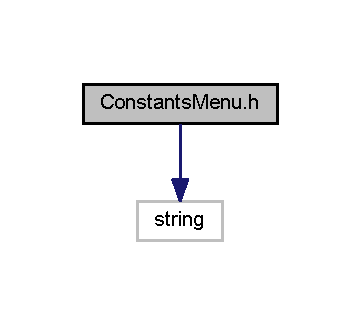
\includegraphics[width=173pt]{_constants_menu_8h__incl}
\end{center}
\end{figure}
Граф файлов, в которые включается этот файл\+:\nopagebreak
\begin{figure}[H]
\begin{center}
\leavevmode
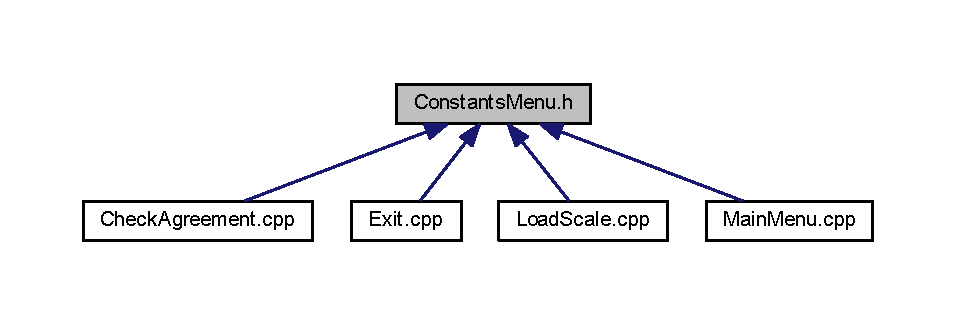
\includegraphics[width=350pt]{_constants_menu_8h__dep__incl}
\end{center}
\end{figure}
\subsection*{Переменные}
\begin{DoxyCompactItemize}
\item 
const std\+::string \hyperlink{_constants_menu_8h_ac0906d6effd5dc68552a724a3edb9330}{menu\+::indentation} = \char`\"{} \char`\"{}
\item 
const std\+::string \hyperlink{_constants_menu_8h_ab9230afa22bdf260e3944290026a5a86}{menu\+::frame\+\_\+left} = \char`\"{} $<$\char`\"{}
\item 
const std\+::string \hyperlink{_constants_menu_8h_a3f786c7ab3caec7dfef9e1fa61b52ae7}{menu\+::frame\+\_\+right} = \char`\"{}$>$ \char`\"{}
\item 
const size\+\_\+t \hyperlink{_constants_menu_8h_aa3bc0d7f62e04dc52dd8f276902448ae}{menu\+::loading\+\_\+size} = 25
\item 
const bool \hyperlink{_constants_menu_8h_aaea5c70964114a416caa58676ddf8066}{menu\+::loading\+\_\+check\+\_\+module} = false
\item 
const size\+\_\+t \hyperlink{_constants_menu_8h_a69bce854c4a150920a5c77eede8cab0a}{menu\+::loading\+\_\+check\+\_\+module\+\_\+sleep} = 1000
\item 
const char \hyperlink{_constants_menu_8h_a56af6a2d586e2b6baa4ebf128a690266}{menu\+::loading\+\_\+left} = \textquotesingle{}\mbox{[}\textquotesingle{}
\item 
const char \hyperlink{_constants_menu_8h_a272b2c0c591457b2aeccaae0c122a1fc}{menu\+::loading\+\_\+right} = \textquotesingle{}\mbox{]}\textquotesingle{}
\item 
const char \hyperlink{_constants_menu_8h_ab79f369195d81dcb241b1ab5269c9d3d}{menu\+::loading\+\_\+progress} = \textquotesingle{}$\vert$\textquotesingle{}
\item 
const char \hyperlink{_constants_menu_8h_ad004c327a8a1c14388a6c7f23d6953a6}{menu\+::loading\+\_\+indenting} = \textquotesingle{} \textquotesingle{}
\end{DoxyCompactItemize}


\subsection{Подробное описание}
Заголовочный файл с константами меню. 

\begin{DoxyAuthor}{Автор}
Sava\+Lione 
\end{DoxyAuthor}


\subsection{Переменные}
\mbox{\Hypertarget{_constants_menu_8h_file_ab9230afa22bdf260e3944290026a5a86}\label{_constants_menu_8h_file_ab9230afa22bdf260e3944290026a5a86}} 
\index{Constants\+Menu.\+h@{Constants\+Menu.\+h}!frame\+\_\+left@{frame\+\_\+left}}
\index{frame\+\_\+left@{frame\+\_\+left}!Constants\+Menu.\+h@{Constants\+Menu.\+h}}
\subsubsection{\texorpdfstring{frame\+\_\+left}{frame\_left}}
{\footnotesize\ttfamily const std\+::string menu\+::frame\+\_\+left = \char`\"{} $<$\char`\"{}}

Левая скобка и отступ слева. \mbox{\Hypertarget{_constants_menu_8h_file_a3f786c7ab3caec7dfef9e1fa61b52ae7}\label{_constants_menu_8h_file_a3f786c7ab3caec7dfef9e1fa61b52ae7}} 
\index{Constants\+Menu.\+h@{Constants\+Menu.\+h}!frame\+\_\+right@{frame\+\_\+right}}
\index{frame\+\_\+right@{frame\+\_\+right}!Constants\+Menu.\+h@{Constants\+Menu.\+h}}
\subsubsection{\texorpdfstring{frame\+\_\+right}{frame\_right}}
{\footnotesize\ttfamily const std\+::string menu\+::frame\+\_\+right = \char`\"{}$>$ \char`\"{}}

Правая скобка и отступ справа. \mbox{\Hypertarget{_constants_menu_8h_file_ac0906d6effd5dc68552a724a3edb9330}\label{_constants_menu_8h_file_ac0906d6effd5dc68552a724a3edb9330}} 
\index{Constants\+Menu.\+h@{Constants\+Menu.\+h}!indentation@{indentation}}
\index{indentation@{indentation}!Constants\+Menu.\+h@{Constants\+Menu.\+h}}
\subsubsection{\texorpdfstring{indentation}{indentation}}
{\footnotesize\ttfamily const std\+::string menu\+::indentation = \char`\"{} \char`\"{}}

Отступ между пунктами меню. \mbox{\Hypertarget{_constants_menu_8h_file_aaea5c70964114a416caa58676ddf8066}\label{_constants_menu_8h_file_aaea5c70964114a416caa58676ddf8066}} 
\index{Constants\+Menu.\+h@{Constants\+Menu.\+h}!loading\+\_\+check\+\_\+module@{loading\+\_\+check\+\_\+module}}
\index{loading\+\_\+check\+\_\+module@{loading\+\_\+check\+\_\+module}!Constants\+Menu.\+h@{Constants\+Menu.\+h}}
\subsubsection{\texorpdfstring{loading\+\_\+check\+\_\+module}{loading\_check\_module}}
{\footnotesize\ttfamily const bool menu\+::loading\+\_\+check\+\_\+module = false}

Включение задержки, для проверки работоспособности модуля загрузки. \mbox{\Hypertarget{_constants_menu_8h_file_a69bce854c4a150920a5c77eede8cab0a}\label{_constants_menu_8h_file_a69bce854c4a150920a5c77eede8cab0a}} 
\index{Constants\+Menu.\+h@{Constants\+Menu.\+h}!loading\+\_\+check\+\_\+module\+\_\+sleep@{loading\+\_\+check\+\_\+module\+\_\+sleep}}
\index{loading\+\_\+check\+\_\+module\+\_\+sleep@{loading\+\_\+check\+\_\+module\+\_\+sleep}!Constants\+Menu.\+h@{Constants\+Menu.\+h}}
\subsubsection{\texorpdfstring{loading\+\_\+check\+\_\+module\+\_\+sleep}{loading\_check\_module\_sleep}}
{\footnotesize\ttfamily const size\+\_\+t menu\+::loading\+\_\+check\+\_\+module\+\_\+sleep = 1000}

Пауза в мс для проверки работоспособности модуля загрузки . \mbox{\Hypertarget{_constants_menu_8h_file_ad004c327a8a1c14388a6c7f23d6953a6}\label{_constants_menu_8h_file_ad004c327a8a1c14388a6c7f23d6953a6}} 
\index{Constants\+Menu.\+h@{Constants\+Menu.\+h}!loading\+\_\+indenting@{loading\+\_\+indenting}}
\index{loading\+\_\+indenting@{loading\+\_\+indenting}!Constants\+Menu.\+h@{Constants\+Menu.\+h}}
\subsubsection{\texorpdfstring{loading\+\_\+indenting}{loading\_indenting}}
{\footnotesize\ttfamily const char menu\+::loading\+\_\+indenting = \textquotesingle{} \textquotesingle{}}

Модуль загрузки. Значение после шкалы прогресса. \mbox{\Hypertarget{_constants_menu_8h_file_a56af6a2d586e2b6baa4ebf128a690266}\label{_constants_menu_8h_file_a56af6a2d586e2b6baa4ebf128a690266}} 
\index{Constants\+Menu.\+h@{Constants\+Menu.\+h}!loading\+\_\+left@{loading\+\_\+left}}
\index{loading\+\_\+left@{loading\+\_\+left}!Constants\+Menu.\+h@{Constants\+Menu.\+h}}
\subsubsection{\texorpdfstring{loading\+\_\+left}{loading\_left}}
{\footnotesize\ttfamily const char menu\+::loading\+\_\+left = \textquotesingle{}\mbox{[}\textquotesingle{}}

Модуль загрузки. Левая скобка. \mbox{\Hypertarget{_constants_menu_8h_file_ab79f369195d81dcb241b1ab5269c9d3d}\label{_constants_menu_8h_file_ab79f369195d81dcb241b1ab5269c9d3d}} 
\index{Constants\+Menu.\+h@{Constants\+Menu.\+h}!loading\+\_\+progress@{loading\+\_\+progress}}
\index{loading\+\_\+progress@{loading\+\_\+progress}!Constants\+Menu.\+h@{Constants\+Menu.\+h}}
\subsubsection{\texorpdfstring{loading\+\_\+progress}{loading\_progress}}
{\footnotesize\ttfamily const char menu\+::loading\+\_\+progress = \textquotesingle{}$\vert$\textquotesingle{}}

Модуль загрузки. Шкала прогресса. \mbox{\Hypertarget{_constants_menu_8h_file_a272b2c0c591457b2aeccaae0c122a1fc}\label{_constants_menu_8h_file_a272b2c0c591457b2aeccaae0c122a1fc}} 
\index{Constants\+Menu.\+h@{Constants\+Menu.\+h}!loading\+\_\+right@{loading\+\_\+right}}
\index{loading\+\_\+right@{loading\+\_\+right}!Constants\+Menu.\+h@{Constants\+Menu.\+h}}
\subsubsection{\texorpdfstring{loading\+\_\+right}{loading\_right}}
{\footnotesize\ttfamily const char menu\+::loading\+\_\+right = \textquotesingle{}\mbox{]}\textquotesingle{}}

Модуль загрузки. Правая скобка. \mbox{\Hypertarget{_constants_menu_8h_file_aa3bc0d7f62e04dc52dd8f276902448ae}\label{_constants_menu_8h_file_aa3bc0d7f62e04dc52dd8f276902448ae}} 
\index{Constants\+Menu.\+h@{Constants\+Menu.\+h}!loading\+\_\+size@{loading\+\_\+size}}
\index{loading\+\_\+size@{loading\+\_\+size}!Constants\+Menu.\+h@{Constants\+Menu.\+h}}
\subsubsection{\texorpdfstring{loading\+\_\+size}{loading\_size}}
{\footnotesize\ttfamily const size\+\_\+t menu\+::loading\+\_\+size = 25}

Размер шкалы модуля загрузки. 
\hypertarget{_exit_8cpp}{}\section{Файл Exit.\+cpp}
\label{_exit_8cpp}\index{Exit.\+cpp@{Exit.\+cpp}}


Модуль выхода из программы.  


{\ttfamily \#include $<$iostream$>$}\newline
{\ttfamily \#include \char`\"{}..\textbackslash{}core\textbackslash{}\+Color.\+h\char`\"{}}\newline
{\ttfamily \#include \char`\"{}..\textbackslash{}core\textbackslash{}\+Logo.\+h\char`\"{}}\newline
{\ttfamily \#include \char`\"{}..\textbackslash{}core\textbackslash{}\+Constants\+Menu.\+h\char`\"{}}\newline
Граф включаемых заголовочных файлов для Exit.\+cpp\+:\nopagebreak
\begin{figure}[H]
\begin{center}
\leavevmode
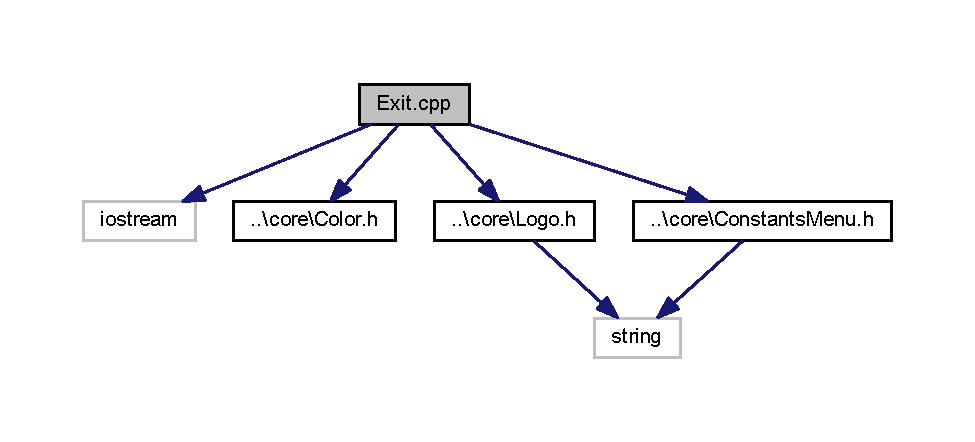
\includegraphics[width=350pt]{_exit_8cpp__incl}
\end{center}
\end{figure}
\subsection*{Функции}
\begin{DoxyCompactItemize}
\item 
void \hyperlink{_exit_8cpp_a540f8b6f2205a3bcf98d2b8f81e8aa09}{v\+\_\+exit} ()
\end{DoxyCompactItemize}


\subsection{Подробное описание}
Модуль выхода из программы. 

\begin{DoxyAuthor}{Автор}
Sava\+Lione 
\end{DoxyAuthor}


\subsection{Функции}
\mbox{\Hypertarget{_exit_8cpp_a540f8b6f2205a3bcf98d2b8f81e8aa09}\label{_exit_8cpp_a540f8b6f2205a3bcf98d2b8f81e8aa09}} 
\index{Exit.\+cpp@{Exit.\+cpp}!v\+\_\+exit@{v\+\_\+exit}}
\index{v\+\_\+exit@{v\+\_\+exit}!Exit.\+cpp@{Exit.\+cpp}}
\subsubsection{\texorpdfstring{v\+\_\+exit()}{v\_exit()}}
{\footnotesize\ttfamily void v\+\_\+exit (\begin{DoxyParamCaption}{ }\end{DoxyParamCaption})}

Вывод текста. Выход из программы. 
\hypertarget{_exit_8h}{}\section{Файл Exit.\+h}
\label{_exit_8h}\index{Exit.\+h@{Exit.\+h}}


Заголовочный файл с подключением модуля выхода из программы.  


Граф файлов, в которые включается этот файл\+:\nopagebreak
\begin{figure}[H]
\begin{center}
\leavevmode
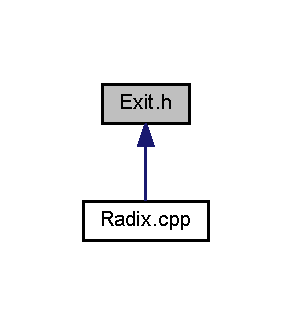
\includegraphics[width=140pt]{_exit_8h__dep__incl}
\end{center}
\end{figure}
\subsection*{Функции}
\begin{DoxyCompactItemize}
\item 
void \hyperlink{_exit_8h_a540f8b6f2205a3bcf98d2b8f81e8aa09}{v\+\_\+exit} ()
\end{DoxyCompactItemize}


\subsection{Подробное описание}
Заголовочный файл с подключением модуля выхода из программы. 

\begin{DoxyAuthor}{Автор}
Sava\+Lione 
\end{DoxyAuthor}


\subsection{Функции}
\mbox{\Hypertarget{_exit_8h_a540f8b6f2205a3bcf98d2b8f81e8aa09}\label{_exit_8h_a540f8b6f2205a3bcf98d2b8f81e8aa09}} 
\index{Exit.\+h@{Exit.\+h}!v\+\_\+exit@{v\+\_\+exit}}
\index{v\+\_\+exit@{v\+\_\+exit}!Exit.\+h@{Exit.\+h}}
\subsubsection{\texorpdfstring{v\+\_\+exit()}{v\_exit()}}
{\footnotesize\ttfamily void v\+\_\+exit (\begin{DoxyParamCaption}{ }\end{DoxyParamCaption})}

Вывод текста. Выход из программы. 
\hypertarget{_initialization_8cpp}{}\section{Файл Initialization.\+cpp}
\label{_initialization_8cpp}\index{Initialization.\+cpp@{Initialization.\+cpp}}


Модуль проверки стандартных файлов программы.  


{\ttfamily \#include $<$fstream$>$}\newline
{\ttfamily \#include \char`\"{}..\textbackslash{}io\textbackslash{}\+Templates.\+h\char`\"{}}\newline
{\ttfamily \#include \char`\"{}..\textbackslash{}io\textbackslash{}\+Logger.\+h\char`\"{}}\newline
{\ttfamily \#include \char`\"{}Constants.\+h\char`\"{}}\newline
{\ttfamily \#include \char`\"{}..\textbackslash{}ui\textbackslash{}\+Load\+Scale.\+h\char`\"{}}\newline
Граф включаемых заголовочных файлов для Initialization.\+cpp\+:
\nopagebreak
\begin{figure}[H]
\begin{center}
\leavevmode
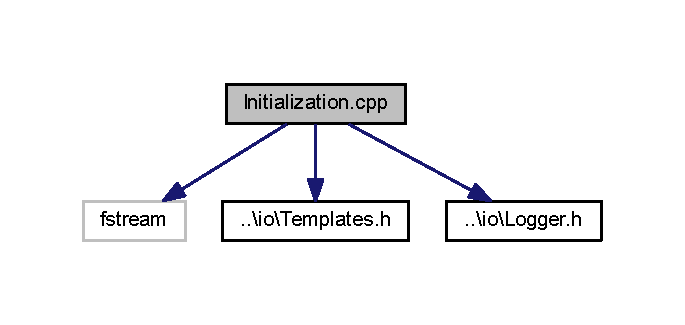
\includegraphics[width=350pt]{_initialization_8cpp__incl}
\end{center}
\end{figure}
\subsection*{Функции}
\begin{DoxyCompactItemize}
\item 
void \hyperlink{_initialization_8cpp_a61271965777637ec3d70f6d7ab0a466a}{v\+\_\+initialization\+\_\+logger\+\_\+log} ()
\begin{DoxyCompactList}\small\item\em Проверка файла logger.\+log. \end{DoxyCompactList}\item 
void \hyperlink{_initialization_8cpp_a86860ef24d9abdaddea8e817e84528a7}{v\+\_\+initialization\+\_\+rules\+\_\+txt} ()
\begin{DoxyCompactList}\small\item\em Проверка файла settings.\+ini. \end{DoxyCompactList}\item 
void \hyperlink{_initialization_8cpp_a9f137f3ae0426a1e7c1a398ad930dc70}{v\+\_\+initialization\+\_\+settings\+\_\+ini} ()
\begin{DoxyCompactList}\small\item\em Проверка файла ip.\+ini. \end{DoxyCompactList}\item 
void \hyperlink{_initialization_8cpp_a64f497032299d5931b86e93305f54f8c}{v\+\_\+initialization\+\_\+ip\+\_\+ini} ()
\begin{DoxyCompactList}\small\item\em Проверка файла rules.\+txt. \end{DoxyCompactList}\item 
void \hyperlink{_initialization_8cpp_a11b373fd61e18cd28810a5b607e1749a}{v\+\_\+initialization} ()
\end{DoxyCompactItemize}


\subsection{Подробное описание}
Модуль проверки стандартных файлов программы. 

Модуль проверяет наличие стандартных файлов программы

Файлы\+: \begin{DoxyVerb}logger.log - вывод логера

rules.txt - правила программы, с которыми должен согласиться пользователь

settings.ini - файл настроек

ip.ini - файл с ip адресами
\end{DoxyVerb}
 \begin{DoxyAuthor}{Автор}
Sava\+Lione 
\end{DoxyAuthor}


\subsection{Функции}
\mbox{\Hypertarget{_initialization_8cpp_a11b373fd61e18cd28810a5b607e1749a}\label{_initialization_8cpp_a11b373fd61e18cd28810a5b607e1749a}} 
\index{Initialization.\+cpp@{Initialization.\+cpp}!v\+\_\+initialization@{v\+\_\+initialization}}
\index{v\+\_\+initialization@{v\+\_\+initialization}!Initialization.\+cpp@{Initialization.\+cpp}}
\subsubsection{\texorpdfstring{v\+\_\+initialization()}{v\_initialization()}}
{\footnotesize\ttfamily void v\+\_\+initialization (\begin{DoxyParamCaption}{ }\end{DoxyParamCaption})}

Главная функция программы

Проверяет наличие 3 стандартных файлов программы \begin{DoxyVerb}logger.log

rules.txt

settings.ini\end{DoxyVerb}
 

См. определение в файле Initialization.\+cpp строка 46

\mbox{\Hypertarget{_initialization_8cpp_a64f497032299d5931b86e93305f54f8c}\label{_initialization_8cpp_a64f497032299d5931b86e93305f54f8c}} 
\index{Initialization.\+cpp@{Initialization.\+cpp}!v\+\_\+initialization\+\_\+ip\+\_\+ini@{v\+\_\+initialization\+\_\+ip\+\_\+ini}}
\index{v\+\_\+initialization\+\_\+ip\+\_\+ini@{v\+\_\+initialization\+\_\+ip\+\_\+ini}!Initialization.\+cpp@{Initialization.\+cpp}}
\subsubsection{\texorpdfstring{v\+\_\+initialization\+\_\+ip\+\_\+ini()}{v\_initialization\_ip\_ini()}}
{\footnotesize\ttfamily void v\+\_\+initialization\+\_\+ip\+\_\+ini (\begin{DoxyParamCaption}{ }\end{DoxyParamCaption})}



Проверка файла rules.\+txt. 

Проверка файла ip.\+ini

При отсутствии файла создаёт его

При наличии файла пропуск

Всё логируется 

См. определение в файле Initialization.\+cpp строка 120

\mbox{\Hypertarget{_initialization_8cpp_a61271965777637ec3d70f6d7ab0a466a}\label{_initialization_8cpp_a61271965777637ec3d70f6d7ab0a466a}} 
\index{Initialization.\+cpp@{Initialization.\+cpp}!v\+\_\+initialization\+\_\+logger\+\_\+log@{v\+\_\+initialization\+\_\+logger\+\_\+log}}
\index{v\+\_\+initialization\+\_\+logger\+\_\+log@{v\+\_\+initialization\+\_\+logger\+\_\+log}!Initialization.\+cpp@{Initialization.\+cpp}}
\subsubsection{\texorpdfstring{v\+\_\+initialization\+\_\+logger\+\_\+log()}{v\_initialization\_logger\_log()}}
{\footnotesize\ttfamily void v\+\_\+initialization\+\_\+logger\+\_\+log (\begin{DoxyParamCaption}{ }\end{DoxyParamCaption})}



Проверка файла logger.\+log. 

Проверка файла logger.\+log

При отсутствии файла создаёт его

При наличии файла пропуск

Всё логируется 

См. определение в файле Initialization.\+cpp строка 70

\mbox{\Hypertarget{_initialization_8cpp_a86860ef24d9abdaddea8e817e84528a7}\label{_initialization_8cpp_a86860ef24d9abdaddea8e817e84528a7}} 
\index{Initialization.\+cpp@{Initialization.\+cpp}!v\+\_\+initialization\+\_\+rules\+\_\+txt@{v\+\_\+initialization\+\_\+rules\+\_\+txt}}
\index{v\+\_\+initialization\+\_\+rules\+\_\+txt@{v\+\_\+initialization\+\_\+rules\+\_\+txt}!Initialization.\+cpp@{Initialization.\+cpp}}
\subsubsection{\texorpdfstring{v\+\_\+initialization\+\_\+rules\+\_\+txt()}{v\_initialization\_rules\_txt()}}
{\footnotesize\ttfamily void v\+\_\+initialization\+\_\+rules\+\_\+txt (\begin{DoxyParamCaption}{ }\end{DoxyParamCaption})}



Проверка файла settings.\+ini. 

Проверка файла rules.\+txt

При отсутствии файла создаёт его

При наличии файла пропуск

Всё логируется 

См. определение в файле Initialization.\+cpp строка 146

\mbox{\Hypertarget{_initialization_8cpp_a9f137f3ae0426a1e7c1a398ad930dc70}\label{_initialization_8cpp_a9f137f3ae0426a1e7c1a398ad930dc70}} 
\index{Initialization.\+cpp@{Initialization.\+cpp}!v\+\_\+initialization\+\_\+settings\+\_\+ini@{v\+\_\+initialization\+\_\+settings\+\_\+ini}}
\index{v\+\_\+initialization\+\_\+settings\+\_\+ini@{v\+\_\+initialization\+\_\+settings\+\_\+ini}!Initialization.\+cpp@{Initialization.\+cpp}}
\subsubsection{\texorpdfstring{v\+\_\+initialization\+\_\+settings\+\_\+ini()}{v\_initialization\_settings\_ini()}}
{\footnotesize\ttfamily void v\+\_\+initialization\+\_\+settings\+\_\+ini (\begin{DoxyParamCaption}{ }\end{DoxyParamCaption})}



Проверка файла ip.\+ini. 

Проверка файла settings.\+ini

При отсутствии файла создаёт его

При наличии файла пропуск

Всё логируется 

См. определение в файле Initialization.\+cpp строка 95


\hypertarget{_initialization_8h}{}\section{Файл Initialization.\+h}
\label{_initialization_8h}\index{Initialization.\+h@{Initialization.\+h}}


Заголовочный файл с вызовом модуля инициализации  


Граф файлов, в которые включается этот файл\+:\nopagebreak
\begin{figure}[H]
\begin{center}
\leavevmode
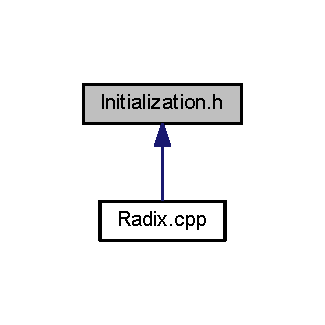
\includegraphics[width=156pt]{_initialization_8h__dep__incl}
\end{center}
\end{figure}
\subsection*{Функции}
\begin{DoxyCompactItemize}
\item 
void \hyperlink{_initialization_8h_a11b373fd61e18cd28810a5b607e1749a}{v\+\_\+initialization} ()
\end{DoxyCompactItemize}


\subsection{Подробное описание}
Заголовочный файл с вызовом модуля инициализации 

Вызов\+: 
\begin{DoxyCode}
\textcolor{keywordtype}{void} \hyperlink{_initialization_8cpp_a11b373fd61e18cd28810a5b607e1749a}{v\_initialization}();
\end{DoxyCode}


\begin{DoxyAuthor}{Автор}
Sava\+Lione 
\end{DoxyAuthor}


\subsection{Функции}
\mbox{\Hypertarget{_initialization_8h_a11b373fd61e18cd28810a5b607e1749a}\label{_initialization_8h_a11b373fd61e18cd28810a5b607e1749a}} 
\index{Initialization.\+h@{Initialization.\+h}!v\+\_\+initialization@{v\+\_\+initialization}}
\index{v\+\_\+initialization@{v\+\_\+initialization}!Initialization.\+h@{Initialization.\+h}}
\subsubsection{\texorpdfstring{v\+\_\+initialization()}{v\_initialization()}}
{\footnotesize\ttfamily void v\+\_\+initialization (\begin{DoxyParamCaption}{ }\end{DoxyParamCaption})}

Главная функция программы

Проверяет наличие 3 стандартных файлов программы \begin{DoxyVerb}logger.log

rules.txt

settings.ini\end{DoxyVerb}
 
\hypertarget{_load_scale_8cpp}{}\section{Файл Load\+Scale.\+cpp}
\label{_load_scale_8cpp}\index{Load\+Scale.\+cpp@{Load\+Scale.\+cpp}}


Модуль вывода шкалы загрузки.  


{\ttfamily \#include $<$iostream$>$}\newline
{\ttfamily \#include $<$windows.\+h$>$}\newline
{\ttfamily \#include \char`\"{}..\textbackslash{}core\textbackslash{}\+Color.\+h\char`\"{}}\newline
{\ttfamily \#include \char`\"{}..\textbackslash{}core\textbackslash{}\+Logo.\+h\char`\"{}}\newline
{\ttfamily \#include \char`\"{}..\textbackslash{}core\textbackslash{}\+Constants\+Menu.\+h\char`\"{}}\newline
Граф включаемых заголовочных файлов для Load\+Scale.\+cpp\+:
\nopagebreak
\begin{figure}[H]
\begin{center}
\leavevmode
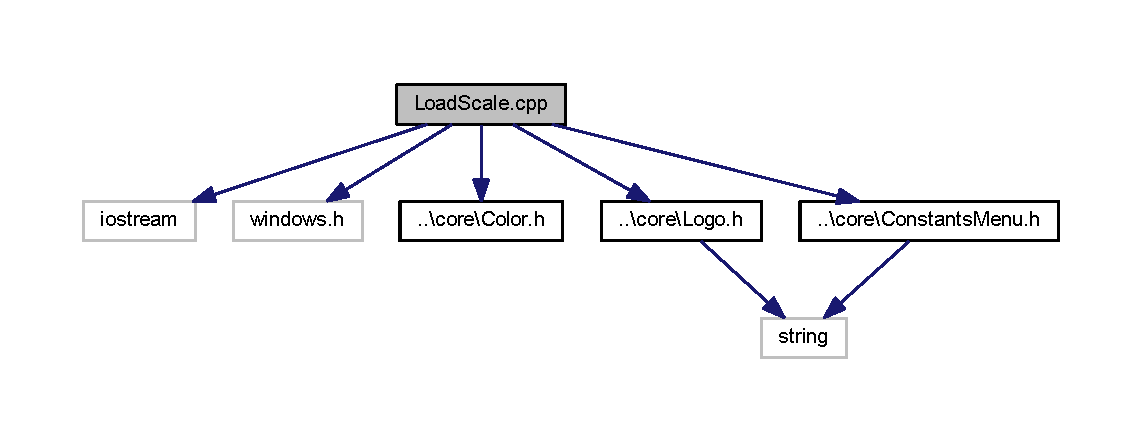
\includegraphics[width=350pt]{_load_scale_8cpp__incl}
\end{center}
\end{figure}
\subsection*{Функции}
\begin{DoxyCompactItemize}
\item 
void \hyperlink{_load_scale_8cpp_ab957e5514a924cccac4e53b2a576d063}{v\+\_\+loadscale} (size\+\_\+t position)
\end{DoxyCompactItemize}


\subsection{Подробное описание}
Модуль вывода шкалы загрузки. 

\begin{DoxyAuthor}{Автор}
Sava\+Lione 
\end{DoxyAuthor}


\subsection{Функции}
\mbox{\Hypertarget{_load_scale_8cpp_ab957e5514a924cccac4e53b2a576d063}\label{_load_scale_8cpp_ab957e5514a924cccac4e53b2a576d063}} 
\index{Load\+Scale.\+cpp@{Load\+Scale.\+cpp}!v\+\_\+loadscale@{v\+\_\+loadscale}}
\index{v\+\_\+loadscale@{v\+\_\+loadscale}!Load\+Scale.\+cpp@{Load\+Scale.\+cpp}}
\subsubsection{\texorpdfstring{v\+\_\+loadscale()}{v\_loadscale()}}
{\footnotesize\ttfamily void v\+\_\+loadscale (\begin{DoxyParamCaption}\item[{size\+\_\+t}]{position }\end{DoxyParamCaption})}

Переключение пунктов меню 
\begin{DoxyParams}[1]{Аргументы}
\mbox{\tt in}  & {\em position} & значение до которого отрисовывать шкалу. \\
\hline
\end{DoxyParams}


См. определение в файле Load\+Scale.\+cpp строка 18


\hypertarget{_load_scale_8h}{}\section{Файл Load\+Scale.\+h}
\label{_load_scale_8h}\index{Load\+Scale.\+h@{Load\+Scale.\+h}}


Заголовочный файл с подключением модуля вывода шкалы загрузки.  


Граф файлов, в которые включается этот файл\+:
\nopagebreak
\begin{figure}[H]
\begin{center}
\leavevmode
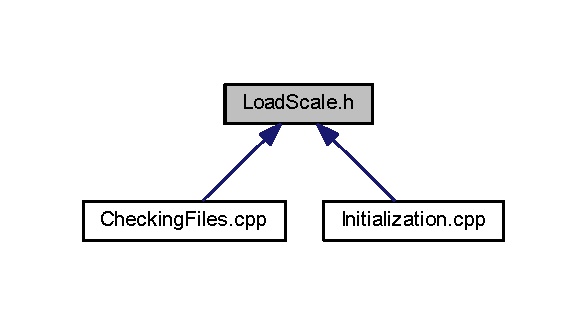
\includegraphics[width=282pt]{_load_scale_8h__dep__incl}
\end{center}
\end{figure}
\subsection*{Функции}
\begin{DoxyCompactItemize}
\item 
void \hyperlink{_load_scale_8h_ab957e5514a924cccac4e53b2a576d063}{v\+\_\+loadscale} (size\+\_\+t position)
\end{DoxyCompactItemize}


\subsection{Подробное описание}
Заголовочный файл с подключением модуля вывода шкалы загрузки. 

\begin{DoxyAuthor}{Автор}
Sava\+Lione 
\end{DoxyAuthor}


\subsection{Функции}
\mbox{\Hypertarget{_load_scale_8h_ab957e5514a924cccac4e53b2a576d063}\label{_load_scale_8h_ab957e5514a924cccac4e53b2a576d063}} 
\index{Load\+Scale.\+h@{Load\+Scale.\+h}!v\+\_\+loadscale@{v\+\_\+loadscale}}
\index{v\+\_\+loadscale@{v\+\_\+loadscale}!Load\+Scale.\+h@{Load\+Scale.\+h}}
\subsubsection{\texorpdfstring{v\+\_\+loadscale()}{v\_loadscale()}}
{\footnotesize\ttfamily void v\+\_\+loadscale (\begin{DoxyParamCaption}\item[{size\+\_\+t}]{position }\end{DoxyParamCaption})}

Переключение пунктов меню 
\begin{DoxyParams}[1]{Аргументы}
\mbox{\tt in}  & {\em position} & значение до которого отрисовывать шкалу. \\
\hline
\end{DoxyParams}


См. определение в файле Load\+Scale.\+cpp строка 19


\hypertarget{_logger_8cpp}{}\section{Файл Logger.\+cpp}
\label{_logger_8cpp}\index{Logger.\+cpp@{Logger.\+cpp}}


Модуль логирования  


{\ttfamily \#include $<$string$>$}\newline
{\ttfamily \#include $<$fstream$>$}\newline
{\ttfamily \#include $<$thread$>$}\newline
{\ttfamily \#include $<$windows.\+h$>$}\newline
{\ttfamily \#include $<$stdio.\+h$>$}\newline
{\ttfamily \#include \char`\"{}Logger.\+h\char`\"{}}\newline
{\ttfamily \#include \char`\"{}Settings.\+h\char`\"{}}\newline
Граф включаемых заголовочных файлов для Logger.\+cpp\+:\nopagebreak
\begin{figure}[H]
\begin{center}
\leavevmode
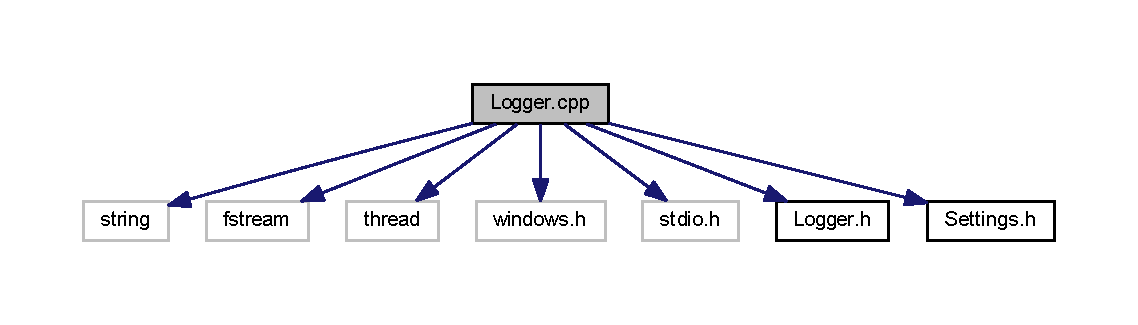
\includegraphics[width=350pt]{_logger_8cpp__incl}
\end{center}
\end{figure}
\subsection*{Функции}
\begin{DoxyCompactItemize}
\item 
void \hyperlink{_logger_8cpp_a37ded7634d8547536bbd135208109766}{log\+\_\+thr} (string \&s, string \&level)
\item 
void \hyperlink{_logger_8cpp_a85cbef1702d055318336f0f3a5036959}{log} (string level, string s)
\end{DoxyCompactItemize}


\subsection{Подробное описание}
Модуль логирования 


\begin{DoxyCode}
Логгер
Логгирование сообщений в файл logger.log
Уровеней лога - 3
Уровень 0:
Вывод сообщений вида:
    [                   ] \{MESSAGE\}
Применение:
    Обработка простых сообщений, без времени и префикса ([PREFIX])
Уровень 1:
Вывод сообщений вида:
    [\{YEAR\}/\{MONTH\}/\{DAY\} \{HOUR\}:\{MINUTE\}:\{SECOND\}] [LOG] \{MESSAGE\}
Применение:
    Обработка простых сообщений(загрузка модуля, отключение модуля, вход в программу, выход из программы и 
      тд.) С временем и префиксом ([LOG])
Уровень 2:
Вывод сообщений вида:
    [\{YEAR\}/\{MONTH\}/\{DAY\} \{HOUR\}:\{MINUTE\}:\{SECOND\}] [WARN] \{MESSAGE\}
Применение:
    Обработка важных сообщений ошибки(не удачная загрузка модуля, не удачный вход в программу, экстренный 
      выход из программы и тд.) С временем и префиксом ([WARN])
\end{DoxyCode}


\begin{DoxyAuthor}{Автор}
Sava\+Lione 
\end{DoxyAuthor}


\subsection{Функции}
\mbox{\Hypertarget{_logger_8cpp_a85cbef1702d055318336f0f3a5036959}\label{_logger_8cpp_a85cbef1702d055318336f0f3a5036959}} 
\index{Logger.\+cpp@{Logger.\+cpp}!log@{log}}
\index{log@{log}!Logger.\+cpp@{Logger.\+cpp}}
\subsubsection{\texorpdfstring{log()}{log()}}
{\footnotesize\ttfamily void log (\begin{DoxyParamCaption}\item[{string}]{level,  }\item[{string}]{s }\end{DoxyParamCaption})}

Логгирование сообщений в файл logger.\+log 
\begin{DoxyParams}[1]{Аргументы}
\mbox{\tt in}  & {\em level} & Уровень логирования \\
\hline
\mbox{\tt in}  & {\em s} & Логируемая информация \\
\hline
\end{DoxyParams}
\mbox{\Hypertarget{_logger_8cpp_a37ded7634d8547536bbd135208109766}\label{_logger_8cpp_a37ded7634d8547536bbd135208109766}} 
\index{Logger.\+cpp@{Logger.\+cpp}!log\+\_\+thr@{log\+\_\+thr}}
\index{log\+\_\+thr@{log\+\_\+thr}!Logger.\+cpp@{Logger.\+cpp}}
\subsubsection{\texorpdfstring{log\+\_\+thr()}{log\_thr()}}
{\footnotesize\ttfamily void log\+\_\+thr (\begin{DoxyParamCaption}\item[{string \&}]{s,  }\item[{string \&}]{level }\end{DoxyParamCaption})}

Функция, для записи лога в файл 
\begin{DoxyParams}[1]{Аргументы}
\mbox{\tt in}  & {\em \&s} & Передача ссылки с сообщением для логирования \\
\hline
\mbox{\tt in}  & {\em \&level} & Передача ссылки с уровнем логирования \\
\hline
\end{DoxyParams}

\hypertarget{_logger_8h}{}\section{Файл Logger.\+h}
\label{_logger_8h}\index{Logger.\+h@{Logger.\+h}}


Заголовочный файл с подключением модуля логирования.  


{\ttfamily \#include $<$string$>$}\newline
Граф включаемых заголовочных файлов для Logger.\+h\+:\nopagebreak
\begin{figure}[H]
\begin{center}
\leavevmode
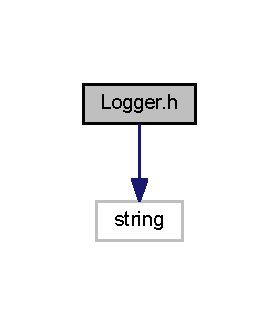
\includegraphics[width=134pt]{_logger_8h__incl}
\end{center}
\end{figure}
Граф файлов, в которые включается этот файл\+:\nopagebreak
\begin{figure}[H]
\begin{center}
\leavevmode
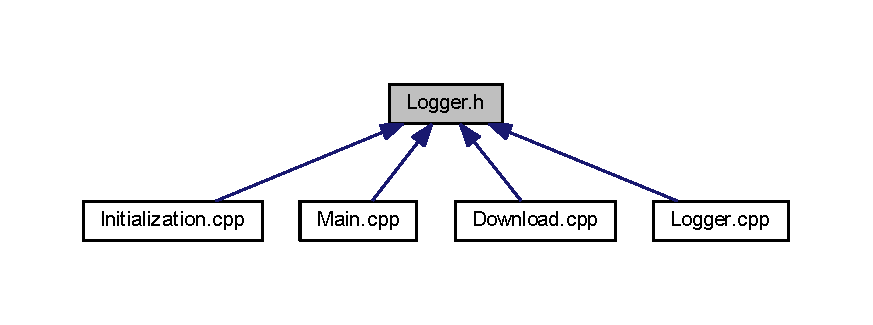
\includegraphics[width=350pt]{_logger_8h__dep__incl}
\end{center}
\end{figure}
\subsection*{Функции}
\begin{DoxyCompactItemize}
\item 
void \hyperlink{_logger_8h_ad35770e66782b0d5c63307682c5de765}{log} (std\+::string level, std\+::string s)
\end{DoxyCompactItemize}


\subsection{Подробное описание}
Заголовочный файл с подключением модуля логирования. 

\begin{DoxyAuthor}{Автор}
Sava\+Lione 
\end{DoxyAuthor}


\subsection{Функции}
\mbox{\Hypertarget{_logger_8h_ad35770e66782b0d5c63307682c5de765}\label{_logger_8h_ad35770e66782b0d5c63307682c5de765}} 
\index{Logger.\+h@{Logger.\+h}!log@{log}}
\index{log@{log}!Logger.\+h@{Logger.\+h}}
\subsubsection{\texorpdfstring{log()}{log()}}
{\footnotesize\ttfamily void log (\begin{DoxyParamCaption}\item[{std\+::string}]{level,  }\item[{std\+::string}]{s }\end{DoxyParamCaption})}

Логгирование сообщений в файл logger.\+log 
\begin{DoxyParams}[1]{Аргументы}
\mbox{\tt in}  & {\em level} & Уровень логирования \\
\hline
\mbox{\tt in}  & {\em s} & Логируемая информация \\
\hline
\end{DoxyParams}

\hypertarget{_logo_8h}{}\section{Файл Logo.\+h}
\label{_logo_8h}\index{Logo.\+h@{Logo.\+h}}


Заголовочный файл с логотипами.  


{\ttfamily \#include $<$string$>$}\newline
Граф включаемых заголовочных файлов для Logo.\+h\+:
\nopagebreak
\begin{figure}[H]
\begin{center}
\leavevmode
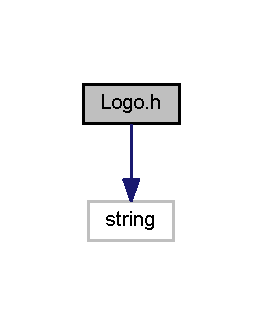
\includegraphics[width=126pt]{_logo_8h__incl}
\end{center}
\end{figure}
Граф файлов, в которые включается этот файл\+:
\nopagebreak
\begin{figure}[H]
\begin{center}
\leavevmode
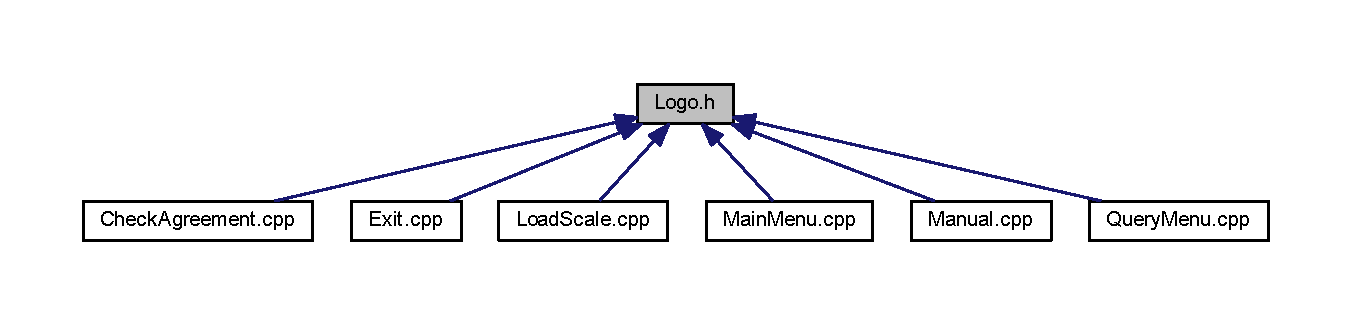
\includegraphics[width=350pt]{_logo_8h__dep__incl}
\end{center}
\end{figure}
\subsection*{Пространства имен}
\begin{DoxyCompactItemize}
\item 
 \hyperlink{namespacelogo}{logo}
\end{DoxyCompactItemize}
\subsection*{Переменные}
\begin{DoxyCompactItemize}
\item 
const std\+::string \hyperlink{namespacelogo_a75fab9a3dcd27565e40b08dbbcbf5e6b}{logo\+::border} = \char`\"{}===========================\textbackslash{}n\char`\"{}
\item 
const std\+::string \hyperlink{namespacelogo_adf18ab31906b644891fc8311df747a9d}{logo\+::little\+\_\+help} = \char`\"{}==== $<$-\/ use to move -\/$>$ ====\textbackslash{}n\char`\"{}
\item 
const std\+::string \hyperlink{namespacelogo_ae5491adc000fde7d3d8229372c877da2}{logo\+::license} = \char`\"{}Do you agree with the license?\textbackslash{}n\char`\"{}
\item 
const std\+::string \hyperlink{namespacelogo_a7570bf74bf945a06ced26f6fccaeab53}{logo\+::move\+\_\+indentation} = \char`\"{} \char`\"{}
\item 
const std\+::string \hyperlink{namespacelogo_a03b6b80b5648e7dbbbf00b258df733b6}{logo\+::move} = \char`\"{}$<$-\/ use to move -\/$>$\textbackslash{}n\char`\"{}
\item 
const std\+::string \hyperlink{namespacelogo_abbbdbfbbcae50e2017f3ed1bdf0e1fa3}{logo\+::radix} = \char`\"{} \+\_\+\+\_\+\+\_\+\+\_\+\+\_\+ \+\_\+ \+\_\+ \textbackslash{}n $\vert$ \+\_\+\+\_\+ \textbackslash{}\textbackslash{} $\vert$ (\+\_\+) \textbackslash{}n $\vert$ $\vert$\+\_\+\+\_\+) $\vert$\+\_\+\+\_\+ \+\_\+ \+\_\+\+\_\+$\vert$ $\vert$\+\_\+\+\_\+\+\_\+ \+\_\+\+\_\+\textbackslash{}n $\vert$ \+\_\+ // \+\_\+` $\vert$/ \+\_\+` $\vert$ \textbackslash{}\textbackslash{} \textbackslash{}\textbackslash{}/ /\textbackslash{}n $\vert$ $\vert$ \textbackslash{}\textbackslash{} \textbackslash{}\textbackslash{} (\+\_\+$\vert$ $\vert$ (\+\_\+$\vert$ $\vert$ $\vert$$>$ $<$ \textbackslash{}n $\vert$\+\_\+$\vert$ \textbackslash{}\textbackslash{}\+\_\+\textbackslash{}\textbackslash{}\+\_\+\+\_\+,\+\_\+$\vert$\textbackslash{}\textbackslash{}\+\_\+\+\_\+,\+\_\+$\vert$\+\_\+/\+\_\+/\textbackslash{}\textbackslash{}\+\_\+\textbackslash{}\textbackslash{} \textbackslash{}n\char`\"{}
\item 
const std\+::string \hyperlink{namespacelogo_ad29ac81055f7eb3624a283f55af8d5ad}{logo\+::loading} = \char`\"{} \+\_\+ \+\_\+ \textbackslash{}n $\vert$ $\vert$ $\vert$ $\vert$\textbackslash{}n $\vert$ $\vert$ \+\_\+\+\_\+\+\_\+ \+\_\+\+\_\+ \+\_\+ \+\_\+\+\_\+$\vert$ $\vert$\textbackslash{}n $\vert$ $\vert$ / \+\_\+ \textbackslash{}\textbackslash{} / \+\_\+` $\vert$/ \+\_\+` $\vert$\textbackslash{}n $\vert$ $\vert$\+\_\+\+\_\+\+\_\+$\vert$ (\+\_\+) $\vert$ (\+\_\+$\vert$ $\vert$ (\+\_\+$\vert$ $\vert$\textbackslash{}n $\vert$\+\_\+\+\_\+\+\_\+\+\_\+\+\_\+\+\_\+\textbackslash{}\textbackslash{}\+\_\+\+\_\+\+\_\+/ \textbackslash{}\textbackslash{}\+\_\+\+\_\+,\+\_\+$\vert$\textbackslash{}\textbackslash{}\+\_\+\+\_\+,\+\_\+$\vert$\textbackslash{}n\char`\"{}
\item 
const std\+::string \hyperlink{namespacelogo_aba8ca66bcf8abe6a0991a13887671863}{logo\+::exit} = \char`\"{} \+\_\+\+\_\+\+\_\+\+\_\+\+\_\+\+\_\+ \+\_\+ \+\_\+ \textbackslash{}n $\vert$ \+\_\+\+\_\+\+\_\+\+\_\+$\vert$ (\+\_\+) $\vert$ \textbackslash{}n $\vert$ $\vert$\+\_\+\+\_\+ \+\_\+\+\_\+ \+\_\+\+\_\+\+\_\+$\vert$ $\vert$\+\_\+ \textbackslash{}n $\vert$ \+\_\+\+\_\+$\vert$ \textbackslash{}\textbackslash{} \textbackslash{}\textbackslash{}/ / $\vert$ \+\_\+\+\_\+$\vert$\textbackslash{}n $\vert$ $\vert$\+\_\+\+\_\+\+\_\+\+\_\+ $>$ $<$$\vert$ $\vert$ $\vert$\+\_\+ \textbackslash{}n $\vert$\+\_\+\+\_\+\+\_\+\+\_\+\+\_\+\+\_\+/\+\_\+/\textbackslash{}\textbackslash{}\+\_\+\textbackslash{}\textbackslash{}\+\_\+$\vert$\textbackslash{}\textbackslash{}\+\_\+\+\_\+$\vert$\textbackslash{}n\char`\"{}
\end{DoxyCompactItemize}


\subsection{Подробное описание}
Заголовочный файл с логотипами. 


\hypertarget{_main_8cpp}{}\section{Файл Main.\+cpp}
\label{_main_8cpp}\index{Main.\+cpp@{Main.\+cpp}}


Главный файл программы  


{\ttfamily \#include $<$Windows.\+h$>$}\newline
{\ttfamily \#include $<$iostream$>$}\newline
{\ttfamily \#include $<$cstring$>$}\newline
{\ttfamily \#include $<$string$>$}\newline
{\ttfamily \#include \char`\"{}..\textbackslash{}io\textbackslash{}\+Settings.\+h\char`\"{}}\newline
{\ttfamily \#include \char`\"{}Radix.\+h\char`\"{}}\newline
{\ttfamily \#include \char`\"{}..\textbackslash{}io\textbackslash{}\+Logger.\+h\char`\"{}}\newline
Граф включаемых заголовочных файлов для Main.\+cpp\+:
\nopagebreak
\begin{figure}[H]
\begin{center}
\leavevmode
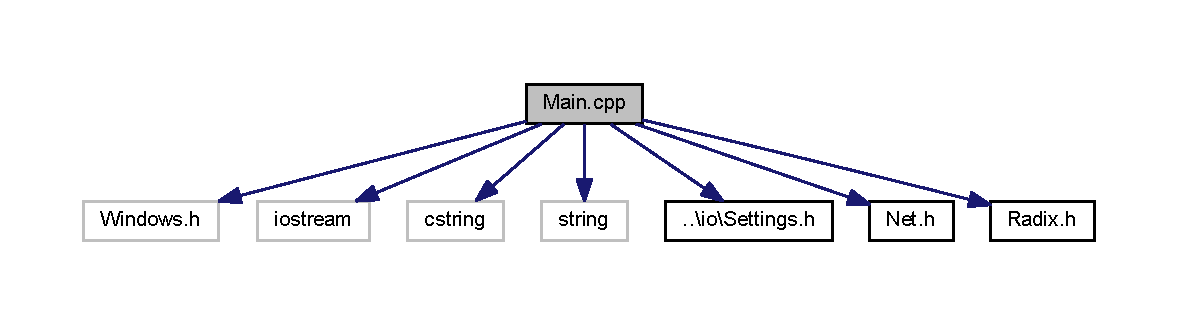
\includegraphics[width=350pt]{_main_8cpp__incl}
\end{center}
\end{figure}
\subsection*{Функции}
\begin{DoxyCompactItemize}
\item 
int \hyperlink{_main_8cpp_ae66f6b31b5ad750f1fe042a706a4e3d4}{main} ()
\end{DoxyCompactItemize}


\subsection{Подробное описание}
Главный файл программы 

\begin{DoxyAuthor}{Автор}
Sava\+Lione 
\end{DoxyAuthor}


\subsection{Функции}
\mbox{\Hypertarget{_main_8cpp_ae66f6b31b5ad750f1fe042a706a4e3d4}\label{_main_8cpp_ae66f6b31b5ad750f1fe042a706a4e3d4}} 
\index{Main.\+cpp@{Main.\+cpp}!main@{main}}
\index{main@{main}!Main.\+cpp@{Main.\+cpp}}
\subsubsection{\texorpdfstring{main()}{main()}}
{\footnotesize\ttfamily int main (\begin{DoxyParamCaption}{ }\end{DoxyParamCaption})}

\begin{DoxyReturn}{Возвращает}
Код завершения программы Вызов программы компилятором 
\end{DoxyReturn}
$<$ Запуск программы 



$<$ Пауза до нажатия любой клавиши 

\begin{Desc}
\item[Примеры\+: ]\par
\hyperlink{log_8cpp-example}{log.\+cpp}.\end{Desc}


См. определение в файле Main.\+cpp строка 23


\hypertarget{_main_menu_8cpp}{}\section{Файл Main\+Menu.\+cpp}
\label{_main_menu_8cpp}\index{Main\+Menu.\+cpp@{Main\+Menu.\+cpp}}


Модуль вывода главного меню программы.  


{\ttfamily \#include $<$iostream$>$}\newline
{\ttfamily \#include $<$conio.\+h$>$}\newline
{\ttfamily \#include $<$string$>$}\newline
{\ttfamily \#include $<$Windows.\+h$>$}\newline
{\ttfamily \#include \char`\"{}..\textbackslash{}core\textbackslash{}\+Color.\+h\char`\"{}}\newline
{\ttfamily \#include \char`\"{}..\textbackslash{}core\textbackslash{}\+Constants\+Menu.\+h\char`\"{}}\newline
{\ttfamily \#include \char`\"{}..\textbackslash{}core\textbackslash{}\+Logo.\+h\char`\"{}}\newline
{\ttfamily \#include \char`\"{}..\textbackslash{}core\textbackslash{}\+A\+D\+B\+\_\+slave.\+h\char`\"{}}\newline
Граф включаемых заголовочных файлов для Main\+Menu.\+cpp\+:
\nopagebreak
\begin{figure}[H]
\begin{center}
\leavevmode
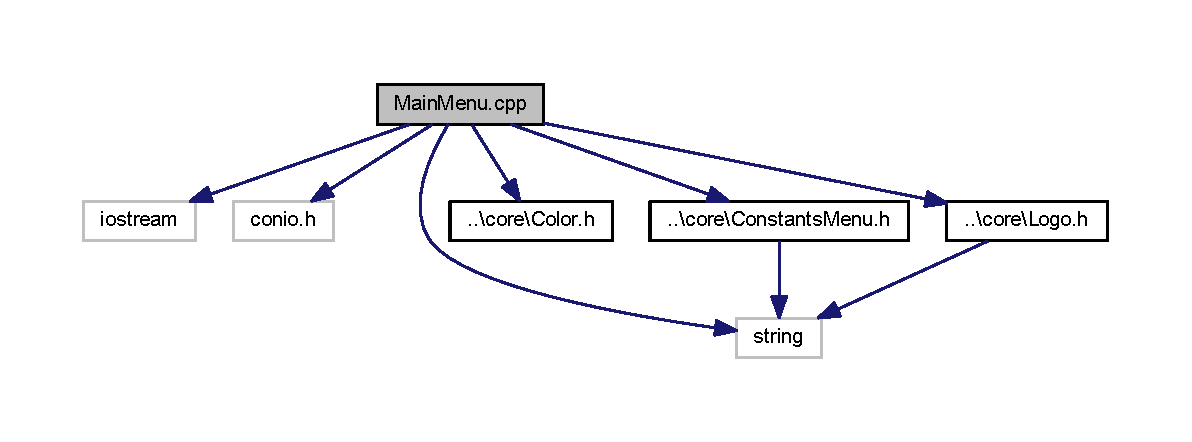
\includegraphics[width=350pt]{_main_menu_8cpp__incl}
\end{center}
\end{figure}
\subsection*{Функции}
\begin{DoxyCompactItemize}
\item 
void \hyperlink{_main_menu_8cpp_ad224308b960ec4f2215ffa68350131f8}{v\+\_\+menu\+\_\+choice} (size\+\_\+t choice)
\item 
void \hyperlink{_main_menu_8cpp_a784c09041cf40075e8eb016a2d8419d6}{root} ()
\item 
int \hyperlink{_main_menu_8cpp_adc9252b438b3b385bf6ccb207688fd4e}{i\+\_\+mainmenu} ()
\end{DoxyCompactItemize}


\subsection{Подробное описание}
Модуль вывода главного меню программы. 

\begin{DoxyAuthor}{Автор}
Sava\+Lione 
\end{DoxyAuthor}


\subsection{Функции}
\mbox{\Hypertarget{_main_menu_8cpp_adc9252b438b3b385bf6ccb207688fd4e}\label{_main_menu_8cpp_adc9252b438b3b385bf6ccb207688fd4e}} 
\index{Main\+Menu.\+cpp@{Main\+Menu.\+cpp}!i\+\_\+mainmenu@{i\+\_\+mainmenu}}
\index{i\+\_\+mainmenu@{i\+\_\+mainmenu}!Main\+Menu.\+cpp@{Main\+Menu.\+cpp}}
\subsubsection{\texorpdfstring{i\+\_\+mainmenu()}{i\_mainmenu()}}
{\footnotesize\ttfamily int i\+\_\+mainmenu (\begin{DoxyParamCaption}{ }\end{DoxyParamCaption})}

Вызов модуля главного меню. \begin{DoxyReturn}{Возвращает}
0 -\/ Выход из программы. 
\end{DoxyReturn}


См. определение в файле Main\+Menu.\+cpp строка 51

\mbox{\Hypertarget{_main_menu_8cpp_a784c09041cf40075e8eb016a2d8419d6}\label{_main_menu_8cpp_a784c09041cf40075e8eb016a2d8419d6}} 
\index{Main\+Menu.\+cpp@{Main\+Menu.\+cpp}!root@{root}}
\index{root@{root}!Main\+Menu.\+cpp@{Main\+Menu.\+cpp}}
\subsubsection{\texorpdfstring{root()}{root()}}
{\footnotesize\ttfamily void root (\begin{DoxyParamCaption}{ }\end{DoxyParamCaption})}

Пункт рутирования телефона. 

См. определение в файле Main\+Menu.\+cpp строка 135

\mbox{\Hypertarget{_main_menu_8cpp_ad224308b960ec4f2215ffa68350131f8}\label{_main_menu_8cpp_ad224308b960ec4f2215ffa68350131f8}} 
\index{Main\+Menu.\+cpp@{Main\+Menu.\+cpp}!v\+\_\+menu\+\_\+choice@{v\+\_\+menu\+\_\+choice}}
\index{v\+\_\+menu\+\_\+choice@{v\+\_\+menu\+\_\+choice}!Main\+Menu.\+cpp@{Main\+Menu.\+cpp}}
\subsubsection{\texorpdfstring{v\+\_\+menu\+\_\+choice()}{v\_menu\_choice()}}
{\footnotesize\ttfamily void v\+\_\+menu\+\_\+choice (\begin{DoxyParamCaption}\item[{size\+\_\+t}]{choice }\end{DoxyParamCaption})}

Переключение пунктов меню 
\begin{DoxyParams}[1]{Аргументы}
\mbox{\tt in}  & {\em choice} & выбор \\
\hline
\end{DoxyParams}


См. определение в файле Main\+Menu.\+cpp строка 24


\hypertarget{_main_menu_8h}{}\section{Файл Main\+Menu.\+h}
\label{_main_menu_8h}\index{Main\+Menu.\+h@{Main\+Menu.\+h}}


Заголовочный файл с подключением модуля главного меню.  


Граф файлов, в которые включается этот файл\+:
\nopagebreak
\begin{figure}[H]
\begin{center}
\leavevmode
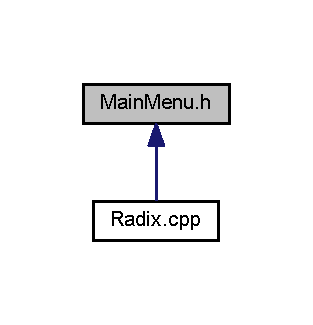
\includegraphics[width=150pt]{_main_menu_8h__dep__incl}
\end{center}
\end{figure}
\subsection*{Функции}
\begin{DoxyCompactItemize}
\item 
int \hyperlink{_main_menu_8h_adc9252b438b3b385bf6ccb207688fd4e}{i\+\_\+mainmenu} ()
\end{DoxyCompactItemize}


\subsection{Подробное описание}
Заголовочный файл с подключением модуля главного меню. 

\begin{DoxyAuthor}{Автор}
Sava\+Lione 
\end{DoxyAuthor}


\subsection{Функции}
\mbox{\Hypertarget{_main_menu_8h_adc9252b438b3b385bf6ccb207688fd4e}\label{_main_menu_8h_adc9252b438b3b385bf6ccb207688fd4e}} 
\index{Main\+Menu.\+h@{Main\+Menu.\+h}!i\+\_\+mainmenu@{i\+\_\+mainmenu}}
\index{i\+\_\+mainmenu@{i\+\_\+mainmenu}!Main\+Menu.\+h@{Main\+Menu.\+h}}
\subsubsection{\texorpdfstring{i\+\_\+mainmenu()}{i\_mainmenu()}}
{\footnotesize\ttfamily int i\+\_\+mainmenu (\begin{DoxyParamCaption}{ }\end{DoxyParamCaption})}

Вызов модуля главного меню. \begin{DoxyReturn}{Возвращает}
0 -\/ Выход из программы. 
\end{DoxyReturn}


См. определение в файле Main\+Menu.\+cpp строка 65


\hypertarget{_radix_8cpp}{}\section{Файл Radix.\+cpp}
\label{_radix_8cpp}\index{Radix.\+cpp@{Radix.\+cpp}}


Главный файл программы  


{\ttfamily \#include \char`\"{}Initialization.\+h\char`\"{}}\newline
Граф включаемых заголовочных файлов для Radix.\+cpp\+:\nopagebreak
\begin{figure}[H]
\begin{center}
\leavevmode
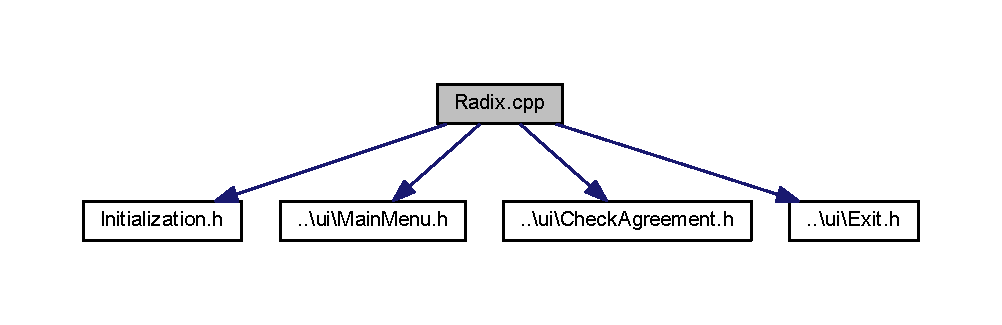
\includegraphics[width=156pt]{_radix_8cpp__incl}
\end{center}
\end{figure}
\subsection*{Функции}
\begin{DoxyCompactItemize}
\item 
void \hyperlink{_radix_8cpp_a86a56c401ce2783ee9288b33af746520}{Radix} ()
\begin{DoxyCompactList}\small\item\em Запуск программы \end{DoxyCompactList}\end{DoxyCompactItemize}


\subsection{Подробное описание}
Главный файл программы 

\begin{DoxyAuthor}{Автор}
Sava\+Lione 
\end{DoxyAuthor}


\subsection{Функции}
\mbox{\Hypertarget{_radix_8cpp_a86a56c401ce2783ee9288b33af746520}\label{_radix_8cpp_a86a56c401ce2783ee9288b33af746520}} 
\index{Radix.\+cpp@{Radix.\+cpp}!Radix@{Radix}}
\index{Radix@{Radix}!Radix.\+cpp@{Radix.\+cpp}}
\subsubsection{\texorpdfstring{Radix()}{Radix()}}
{\footnotesize\ttfamily void Radix (\begin{DoxyParamCaption}{ }\end{DoxyParamCaption})}



Запуск программы 

Запуск модуля инициализации 
\hypertarget{_radix_8h}{}\section{Файл Radix.\+h}
\label{_radix_8h}\index{Radix.\+h@{Radix.\+h}}


Заголовочный файл с вызовом главной функции программы  


Граф файлов, в которые включается этот файл\+:
\nopagebreak
\begin{figure}[H]
\begin{center}
\leavevmode
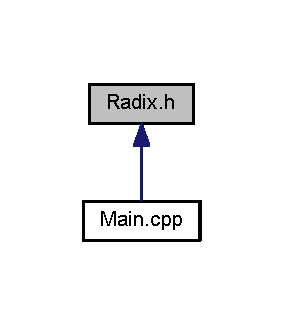
\includegraphics[width=136pt]{d6/db2/_radix_8h__dep__incl}
\end{center}
\end{figure}
\subsection*{Функции}
\begin{DoxyCompactItemize}
\item 
void \hyperlink{_radix_8h_a86a56c401ce2783ee9288b33af746520}{Radix} ()
\begin{DoxyCompactList}\small\item\em Запуск программы \end{DoxyCompactList}\end{DoxyCompactItemize}


\subsection{Подробное описание}
Заголовочный файл с вызовом главной функции программы 

\begin{DoxyAuthor}{Автор}
Sava\+Lione 
\end{DoxyAuthor}


\subsection{Функции}
\mbox{\Hypertarget{_radix_8h_a86a56c401ce2783ee9288b33af746520}\label{_radix_8h_a86a56c401ce2783ee9288b33af746520}} 
\index{Radix.\+h@{Radix.\+h}!Radix@{Radix}}
\index{Radix@{Radix}!Radix.\+h@{Radix.\+h}}
\subsubsection{\texorpdfstring{Radix()}{Radix()}}
{\footnotesize\ttfamily void Radix (\begin{DoxyParamCaption}{ }\end{DoxyParamCaption})}



Запуск программы 

$<$ Запуск модуля инициализации 
\hypertarget{_rules_list_8cpp}{}\section{Файл Rules\+List.\+cpp}
\label{_rules_list_8cpp}\index{Rules\+List.\+cpp@{Rules\+List.\+cpp}}


Модуль чтения правил.  


{\ttfamily \#include $<$fstream$>$}\newline
{\ttfamily \#include $<$string$>$}\newline
{\ttfamily \#include \char`\"{}../core/\+Constants.\+h\char`\"{}}\newline
Граф включаемых заголовочных файлов для Rules\+List.\+cpp\+:\nopagebreak
\begin{figure}[H]
\begin{center}
\leavevmode
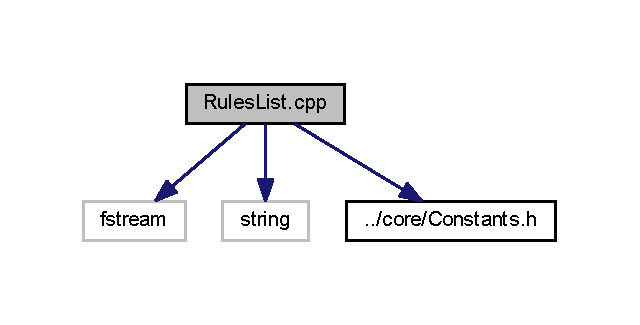
\includegraphics[width=307pt]{_rules_list_8cpp__incl}
\end{center}
\end{figure}
\subsection*{Функции}
\begin{DoxyCompactItemize}
\item 
string \hyperlink{_rules_list_8cpp_a7c6f9bd6ee5089b03c66028f99271e15}{s\+\_\+ruleslist} ()
\end{DoxyCompactItemize}


\subsection{Подробное описание}
Модуль чтения правил. 

\begin{DoxyAuthor}{Автор}
Sava\+Lione 
\end{DoxyAuthor}


\subsection{Функции}
\mbox{\Hypertarget{_rules_list_8cpp_a7c6f9bd6ee5089b03c66028f99271e15}\label{_rules_list_8cpp_a7c6f9bd6ee5089b03c66028f99271e15}} 
\index{Rules\+List.\+cpp@{Rules\+List.\+cpp}!s\+\_\+ruleslist@{s\+\_\+ruleslist}}
\index{s\+\_\+ruleslist@{s\+\_\+ruleslist}!Rules\+List.\+cpp@{Rules\+List.\+cpp}}
\subsubsection{\texorpdfstring{s\+\_\+ruleslist()}{s\_ruleslist()}}
{\footnotesize\ttfamily string s\+\_\+ruleslist (\begin{DoxyParamCaption}{ }\end{DoxyParamCaption})}

Чтение правил программы \begin{DoxyReturn}{Возвращает}
строка с правилами 
\end{DoxyReturn}

\hypertarget{_rules_list_8h}{}\section{Файл Rules\+List.\+h}
\label{_rules_list_8h}\index{Rules\+List.\+h@{Rules\+List.\+h}}


Заголовочный файл с подключением модуля чтения правил.  


{\ttfamily \#include $<$string$>$}\newline
Граф включаемых заголовочных файлов для Rules\+List.\+h\+:
\nopagebreak
\begin{figure}[H]
\begin{center}
\leavevmode
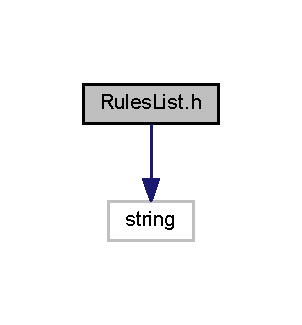
\includegraphics[width=145pt]{_rules_list_8h__incl}
\end{center}
\end{figure}
Граф файлов, в которые включается этот файл\+:
\nopagebreak
\begin{figure}[H]
\begin{center}
\leavevmode
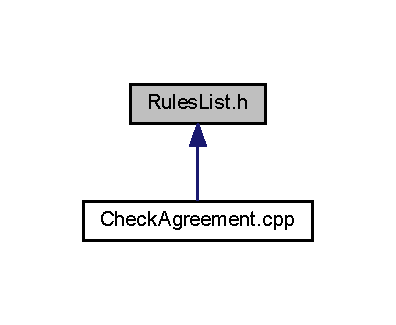
\includegraphics[width=190pt]{_rules_list_8h__dep__incl}
\end{center}
\end{figure}
\subsection*{Функции}
\begin{DoxyCompactItemize}
\item 
std\+::string \hyperlink{_rules_list_8h_a5010d1a6599fe48d9bd963375613da92}{s\+\_\+ruleslist} ()
\end{DoxyCompactItemize}


\subsection{Подробное описание}
Заголовочный файл с подключением модуля чтения правил. 

\begin{DoxyAuthor}{Автор}
Sava\+Lione 
\end{DoxyAuthor}


\subsection{Функции}
\mbox{\Hypertarget{_rules_list_8h_a5010d1a6599fe48d9bd963375613da92}\label{_rules_list_8h_a5010d1a6599fe48d9bd963375613da92}} 
\index{Rules\+List.\+h@{Rules\+List.\+h}!s\+\_\+ruleslist@{s\+\_\+ruleslist}}
\index{s\+\_\+ruleslist@{s\+\_\+ruleslist}!Rules\+List.\+h@{Rules\+List.\+h}}
\subsubsection{\texorpdfstring{s\+\_\+ruleslist()}{s\_ruleslist()}}
{\footnotesize\ttfamily std\+::string s\+\_\+ruleslist (\begin{DoxyParamCaption}{ }\end{DoxyParamCaption})}

Чтение правил программы \begin{DoxyReturn}{Возвращает}
строка с правилами 
\end{DoxyReturn}


См. определение в файле Rules\+List.\+cpp строка 16


\hypertarget{_settings_8cpp}{}\section{Файл Settings.\+cpp}
\label{_settings_8cpp}\index{Settings.\+cpp@{Settings.\+cpp}}


Модуль настроек. Парсит переменные в файлах  


{\ttfamily \#include $<$fstream$>$}\newline
{\ttfamily \#include $<$string$>$}\newline
{\ttfamily \#include \char`\"{}../core/\+Constants.\+h\char`\"{}}\newline
Граф включаемых заголовочных файлов для Settings.\+cpp\+:\nopagebreak
\begin{figure}[H]
\begin{center}
\leavevmode
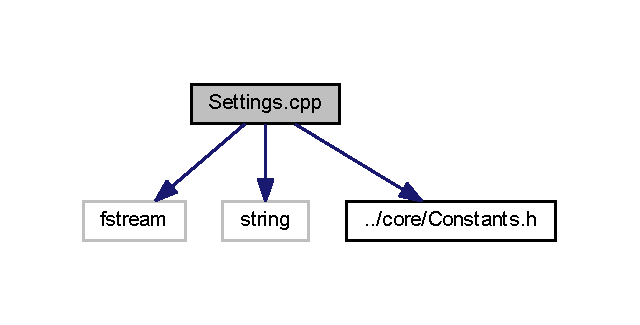
\includegraphics[width=307pt]{_settings_8cpp__incl}
\end{center}
\end{figure}
\subsection*{Функции}
\begin{DoxyCompactItemize}
\item 
bool \hyperlink{_settings_8cpp_a7fcd42142e325cb27a380f49d655f9de}{b\+\_\+settings} (char ch\+\_\+arr\+\_\+value\mbox{[}$\,$\mbox{]})
\end{DoxyCompactItemize}


\subsection{Подробное описание}
Модуль настроек. Парсит переменные в файлах 

\begin{DoxyAuthor}{Автор}
Sava\+Lione 
\end{DoxyAuthor}


\subsection{Функции}
\mbox{\Hypertarget{_settings_8cpp_a7fcd42142e325cb27a380f49d655f9de}\label{_settings_8cpp_a7fcd42142e325cb27a380f49d655f9de}} 
\index{Settings.\+cpp@{Settings.\+cpp}!b\+\_\+settings@{b\+\_\+settings}}
\index{b\+\_\+settings@{b\+\_\+settings}!Settings.\+cpp@{Settings.\+cpp}}
\subsubsection{\texorpdfstring{b\+\_\+settings()}{b\_settings()}}
{\footnotesize\ttfamily bool b\+\_\+settings (\begin{DoxyParamCaption}\item[{char}]{ch\+\_\+arr\+\_\+value\mbox{[}$\,$\mbox{]} }\end{DoxyParamCaption})}

Парсинг параметров 
\begin{DoxyParams}[1]{Аргументы}
\mbox{\tt in}  & {\em ch\+\_\+arr\+\_\+value\mbox{[}$\,$\mbox{]}} & Значение, которое надо найти в файле \\
\hline
\end{DoxyParams}
\begin{DoxyReturn}{Возвращает}
Значение переменной true false 
\end{DoxyReturn}

\hypertarget{_settings_8h}{}\section{Файл Settings.\+h}
\label{_settings_8h}\index{Settings.\+h@{Settings.\+h}}


Заголовочный файл с подключением модуля настроек.  


Граф файлов, в которые включается этот файл\+:\nopagebreak
\begin{figure}[H]
\begin{center}
\leavevmode
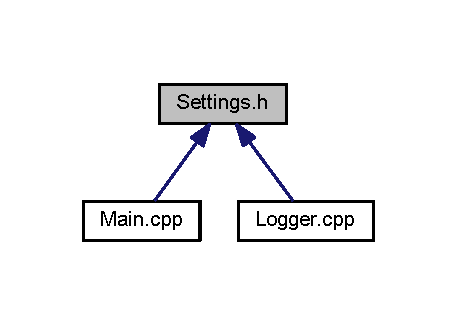
\includegraphics[width=220pt]{_settings_8h__dep__incl}
\end{center}
\end{figure}
\subsection*{Функции}
\begin{DoxyCompactItemize}
\item 
bool \hyperlink{_settings_8h_a7fcd42142e325cb27a380f49d655f9de}{b\+\_\+settings} (char ch\+\_\+arr\+\_\+value\mbox{[}$\,$\mbox{]})
\item 
void \hyperlink{_settings_8h_a8922c0342039e2f0d376c1d806eb84d2}{v\+\_\+get\+\_\+ip} (char $\ast$ch\+\_\+return)
\end{DoxyCompactItemize}


\subsection{Подробное описание}
Заголовочный файл с подключением модуля настроек. 

\begin{DoxyAuthor}{Автор}
Sava\+Lione 
\end{DoxyAuthor}


\subsection{Функции}
\mbox{\Hypertarget{_settings_8h_a7fcd42142e325cb27a380f49d655f9de}\label{_settings_8h_a7fcd42142e325cb27a380f49d655f9de}} 
\index{Settings.\+h@{Settings.\+h}!b\+\_\+settings@{b\+\_\+settings}}
\index{b\+\_\+settings@{b\+\_\+settings}!Settings.\+h@{Settings.\+h}}
\subsubsection{\texorpdfstring{b\+\_\+settings()}{b\_settings()}}
{\footnotesize\ttfamily bool b\+\_\+settings (\begin{DoxyParamCaption}\item[{char}]{ch\+\_\+arr\+\_\+value\mbox{[}$\,$\mbox{]} }\end{DoxyParamCaption})}

Парсинг параметров 
\begin{DoxyParams}[1]{Аргументы}
\mbox{\tt in}  & {\em ch\+\_\+arr\+\_\+value\mbox{[}$\,$\mbox{]}} & Значение, которое надо найти в файле \\
\hline
\end{DoxyParams}
\begin{DoxyReturn}{Возвращает}
Значение переменной true false 
\end{DoxyReturn}
\mbox{\Hypertarget{_settings_8h_a8922c0342039e2f0d376c1d806eb84d2}\label{_settings_8h_a8922c0342039e2f0d376c1d806eb84d2}} 
\index{Settings.\+h@{Settings.\+h}!v\+\_\+get\+\_\+ip@{v\+\_\+get\+\_\+ip}}
\index{v\+\_\+get\+\_\+ip@{v\+\_\+get\+\_\+ip}!Settings.\+h@{Settings.\+h}}
\subsubsection{\texorpdfstring{v\+\_\+get\+\_\+ip()}{v\_get\_ip()}}
{\footnotesize\ttfamily void v\+\_\+get\+\_\+ip (\begin{DoxyParamCaption}\item[{char $\ast$}]{ch\+\_\+return }\end{DoxyParamCaption})}

Парсинг ip адресов 
\begin{DoxyParams}[1]{Аргументы}
\mbox{\tt out}  & {\em ch\+\_\+return} & Массив char, в который запишется ip адрес \\
\hline
\end{DoxyParams}
\begin{DoxyReturn}{Возвращает}
Массив символов, который запишется в ch\+\_\+return 
\end{DoxyReturn}

\hypertarget{_standards_8cpp}{}\section{Файл Standards.\+cpp}
\label{_standards_8cpp}\index{Standards.\+cpp@{Standards.\+cpp}}

\hypertarget{_templates_8cpp}{}\section{Файл Templates.\+cpp}
\label{_templates_8cpp}\index{Templates.\+cpp@{Templates.\+cpp}}


Функции для создания стандартных файлов программы.  


{\ttfamily \#include $<$fstream$>$}\newline
{\ttfamily \#include \char`\"{}Templates.\+h\char`\"{}}\newline
{\ttfamily \#include \char`\"{}..\textbackslash{}core\textbackslash{}\+Constants.\+h\char`\"{}}\newline
Граф включаемых заголовочных файлов для Templates.\+cpp\+:
\nopagebreak
\begin{figure}[H]
\begin{center}
\leavevmode
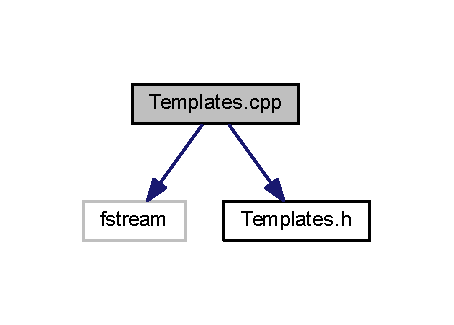
\includegraphics[width=336pt]{_templates_8cpp__incl}
\end{center}
\end{figure}
\subsection*{Функции}
\begin{DoxyCompactItemize}
\item 
void \hyperlink{_templates_8cpp_abeb0b4d4d31b9c74744a0b9881d95066}{v\+\_\+templates\+\_\+create\+\_\+logger\+\_\+log} ()
\item 
void \hyperlink{_templates_8cpp_afbd4b91587b894d5e8b6ea50209ed5dc}{v\+\_\+templates\+\_\+create\+\_\+rules\+\_\+txt} ()
\item 
void \hyperlink{_templates_8cpp_a593e33d5988d6a49d581f52d94471895}{v\+\_\+templates\+\_\+create\+\_\+settings\+\_\+ini} ()
\item 
void \hyperlink{_templates_8cpp_a4cdca62a0922d9ad016c50f1251636cb}{v\+\_\+templates\+\_\+create\+\_\+ip\+\_\+ini} ()
\end{DoxyCompactItemize}


\subsection{Подробное описание}
Функции для создания стандартных файлов программы. 

\begin{DoxyAuthor}{Автор}
Sava\+Lione 
\end{DoxyAuthor}


\subsection{Функции}
\mbox{\Hypertarget{_templates_8cpp_a4cdca62a0922d9ad016c50f1251636cb}\label{_templates_8cpp_a4cdca62a0922d9ad016c50f1251636cb}} 
\index{Templates.\+cpp@{Templates.\+cpp}!v\+\_\+templates\+\_\+create\+\_\+ip\+\_\+ini@{v\+\_\+templates\+\_\+create\+\_\+ip\+\_\+ini}}
\index{v\+\_\+templates\+\_\+create\+\_\+ip\+\_\+ini@{v\+\_\+templates\+\_\+create\+\_\+ip\+\_\+ini}!Templates.\+cpp@{Templates.\+cpp}}
\subsubsection{\texorpdfstring{v\+\_\+templates\+\_\+create\+\_\+ip\+\_\+ini()}{v\_templates\_create\_ip\_ini()}}
{\footnotesize\ttfamily void v\+\_\+templates\+\_\+create\+\_\+ip\+\_\+ini (\begin{DoxyParamCaption}{ }\end{DoxyParamCaption})}

Создание файла ip. \begin{DoxyVerb}ip.ini - файл с ip адресами\end{DoxyVerb}
 

См. определение в файле Templates.\+cpp строка 83

\mbox{\Hypertarget{_templates_8cpp_abeb0b4d4d31b9c74744a0b9881d95066}\label{_templates_8cpp_abeb0b4d4d31b9c74744a0b9881d95066}} 
\index{Templates.\+cpp@{Templates.\+cpp}!v\+\_\+templates\+\_\+create\+\_\+logger\+\_\+log@{v\+\_\+templates\+\_\+create\+\_\+logger\+\_\+log}}
\index{v\+\_\+templates\+\_\+create\+\_\+logger\+\_\+log@{v\+\_\+templates\+\_\+create\+\_\+logger\+\_\+log}!Templates.\+cpp@{Templates.\+cpp}}
\subsubsection{\texorpdfstring{v\+\_\+templates\+\_\+create\+\_\+logger\+\_\+log()}{v\_templates\_create\_logger\_log()}}
{\footnotesize\ttfamily void v\+\_\+templates\+\_\+create\+\_\+logger\+\_\+log (\begin{DoxyParamCaption}{ }\end{DoxyParamCaption})}

Создание файла пользовательского соглашения. \begin{DoxyVerb}logger.log - файл с логом вывода\end{DoxyVerb}
 

См. определение в файле Templates.\+cpp строка 21

\mbox{\Hypertarget{_templates_8cpp_afbd4b91587b894d5e8b6ea50209ed5dc}\label{_templates_8cpp_afbd4b91587b894d5e8b6ea50209ed5dc}} 
\index{Templates.\+cpp@{Templates.\+cpp}!v\+\_\+templates\+\_\+create\+\_\+rules\+\_\+txt@{v\+\_\+templates\+\_\+create\+\_\+rules\+\_\+txt}}
\index{v\+\_\+templates\+\_\+create\+\_\+rules\+\_\+txt@{v\+\_\+templates\+\_\+create\+\_\+rules\+\_\+txt}!Templates.\+cpp@{Templates.\+cpp}}
\subsubsection{\texorpdfstring{v\+\_\+templates\+\_\+create\+\_\+rules\+\_\+txt()}{v\_templates\_create\_rules\_txt()}}
{\footnotesize\ttfamily void v\+\_\+templates\+\_\+create\+\_\+rules\+\_\+txt (\begin{DoxyParamCaption}{ }\end{DoxyParamCaption})}

Создание файла пользовательского соглашения. \begin{DoxyVerb}rules.txt - файл с пользовательским соглашением\end{DoxyVerb}
 

См. определение в файле Templates.\+cpp строка 38

\mbox{\Hypertarget{_templates_8cpp_a593e33d5988d6a49d581f52d94471895}\label{_templates_8cpp_a593e33d5988d6a49d581f52d94471895}} 
\index{Templates.\+cpp@{Templates.\+cpp}!v\+\_\+templates\+\_\+create\+\_\+settings\+\_\+ini@{v\+\_\+templates\+\_\+create\+\_\+settings\+\_\+ini}}
\index{v\+\_\+templates\+\_\+create\+\_\+settings\+\_\+ini@{v\+\_\+templates\+\_\+create\+\_\+settings\+\_\+ini}!Templates.\+cpp@{Templates.\+cpp}}
\subsubsection{\texorpdfstring{v\+\_\+templates\+\_\+create\+\_\+settings\+\_\+ini()}{v\_templates\_create\_settings\_ini()}}
{\footnotesize\ttfamily void v\+\_\+templates\+\_\+create\+\_\+settings\+\_\+ini (\begin{DoxyParamCaption}{ }\end{DoxyParamCaption})}

Создание файла настроек. \begin{DoxyVerb}settings.ini - файл с настройками\end{DoxyVerb}
 

См. определение в файле Templates.\+cpp строка 59


\hypertarget{_templates_8h}{}\section{Файл Templates.\+h}
\label{_templates_8h}\index{Templates.\+h@{Templates.\+h}}


Заголовочный файл с подключением модуля создания стандартных файлов программы.  


Граф файлов, в которые включается этот файл\+:
\nopagebreak
\begin{figure}[H]
\begin{center}
\leavevmode
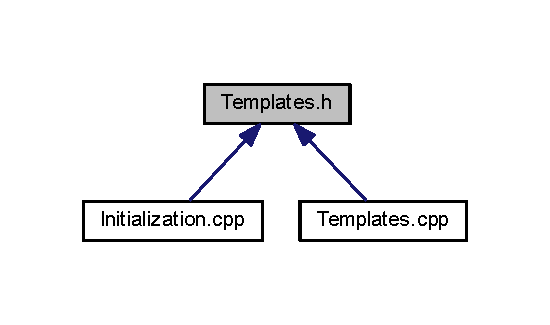
\includegraphics[width=264pt]{_templates_8h__dep__incl}
\end{center}
\end{figure}
\subsection*{Функции}
\begin{DoxyCompactItemize}
\item 
void \hyperlink{_templates_8h_abeb0b4d4d31b9c74744a0b9881d95066}{v\+\_\+templates\+\_\+create\+\_\+logger\+\_\+log} ()
\item 
void \hyperlink{_templates_8h_afbd4b91587b894d5e8b6ea50209ed5dc}{v\+\_\+templates\+\_\+create\+\_\+rules\+\_\+txt} ()
\item 
void \hyperlink{_templates_8h_a593e33d5988d6a49d581f52d94471895}{v\+\_\+templates\+\_\+create\+\_\+settings\+\_\+ini} ()
\end{DoxyCompactItemize}


\subsection{Подробное описание}
Заголовочный файл с подключением модуля создания стандартных файлов программы. 

\begin{DoxyAuthor}{Автор}
Sava\+Lione 
\end{DoxyAuthor}


\subsection{Функции}
\mbox{\Hypertarget{_templates_8h_abeb0b4d4d31b9c74744a0b9881d95066}\label{_templates_8h_abeb0b4d4d31b9c74744a0b9881d95066}} 
\index{Templates.\+h@{Templates.\+h}!v\+\_\+templates\+\_\+create\+\_\+logger\+\_\+log@{v\+\_\+templates\+\_\+create\+\_\+logger\+\_\+log}}
\index{v\+\_\+templates\+\_\+create\+\_\+logger\+\_\+log@{v\+\_\+templates\+\_\+create\+\_\+logger\+\_\+log}!Templates.\+h@{Templates.\+h}}
\subsubsection{\texorpdfstring{v\+\_\+templates\+\_\+create\+\_\+logger\+\_\+log()}{v\_templates\_create\_logger\_log()}}
{\footnotesize\ttfamily void v\+\_\+templates\+\_\+create\+\_\+logger\+\_\+log (\begin{DoxyParamCaption}{ }\end{DoxyParamCaption})}

Создание файла пользовательского соглашения. \begin{DoxyVerb}logger.log - файл с логом вывода\end{DoxyVerb}
 

См. определение в файле Templates.\+cpp строка 21

\mbox{\Hypertarget{_templates_8h_afbd4b91587b894d5e8b6ea50209ed5dc}\label{_templates_8h_afbd4b91587b894d5e8b6ea50209ed5dc}} 
\index{Templates.\+h@{Templates.\+h}!v\+\_\+templates\+\_\+create\+\_\+rules\+\_\+txt@{v\+\_\+templates\+\_\+create\+\_\+rules\+\_\+txt}}
\index{v\+\_\+templates\+\_\+create\+\_\+rules\+\_\+txt@{v\+\_\+templates\+\_\+create\+\_\+rules\+\_\+txt}!Templates.\+h@{Templates.\+h}}
\subsubsection{\texorpdfstring{v\+\_\+templates\+\_\+create\+\_\+rules\+\_\+txt()}{v\_templates\_create\_rules\_txt()}}
{\footnotesize\ttfamily void v\+\_\+templates\+\_\+create\+\_\+rules\+\_\+txt (\begin{DoxyParamCaption}{ }\end{DoxyParamCaption})}

Создание файла пользовательского соглашения. \begin{DoxyVerb}rules.txt - файл с пользовательским соглашением\end{DoxyVerb}
 

См. определение в файле Templates.\+cpp строка 38

\mbox{\Hypertarget{_templates_8h_a593e33d5988d6a49d581f52d94471895}\label{_templates_8h_a593e33d5988d6a49d581f52d94471895}} 
\index{Templates.\+h@{Templates.\+h}!v\+\_\+templates\+\_\+create\+\_\+settings\+\_\+ini@{v\+\_\+templates\+\_\+create\+\_\+settings\+\_\+ini}}
\index{v\+\_\+templates\+\_\+create\+\_\+settings\+\_\+ini@{v\+\_\+templates\+\_\+create\+\_\+settings\+\_\+ini}!Templates.\+h@{Templates.\+h}}
\subsubsection{\texorpdfstring{v\+\_\+templates\+\_\+create\+\_\+settings\+\_\+ini()}{v\_templates\_create\_settings\_ini()}}
{\footnotesize\ttfamily void v\+\_\+templates\+\_\+create\+\_\+settings\+\_\+ini (\begin{DoxyParamCaption}{ }\end{DoxyParamCaption})}

Создание файла настроек. \begin{DoxyVerb}settings.ini - файл с настройками\end{DoxyVerb}
 

См. определение в файле Templates.\+cpp строка 59


\chapter{Примеры}
\hypertarget{log_8cpp-example}{}\section{log.\+cpp}
\begin{DoxyAuthor}{Автор}
Sava\+Lione
\end{DoxyAuthor}

\begin{DoxyCodeInclude}
\textcolor{preprocessor}{#include "..\(\backslash\)io\(\backslash\)Logger.h"}

\textcolor{keywordtype}{int} \hyperlink{_main_8cpp_ae66f6b31b5ad750f1fe042a706a4e3d4}{main}() \{
    \hyperlink{_logger_8cpp_a85cbef1702d055318336f0f3a5036959}{log}(\textcolor{stringliteral}{"LOG"}, \textcolor{stringliteral}{"Hello World!!!"});
    \textcolor{keywordflow}{return} 0;
\}
\end{DoxyCodeInclude}
 
%--- End generated contents ---

% Index
\backmatter
\newpage
\phantomsection
\clearemptydoublepage
\addcontentsline{toc}{chapter}{Алфавитный указатель}
\printindex

\end{document}
